\begin{name}
    {\tenchude}
    {\tendethi}
    {Toán thầy Phát}
    {\thoigian}
\end{name}
\setcounter{ex}{0}\setcounter{bt}{0}
\Opensolutionfile{ans}[ans/ans-2-GHK1-7-VietDuc-HaNoi-20]

\begin{ex}%[Đề GHK1 môn Toán 12 THPT Việt Đức, Hà Nội, 2019-2020]%[Trần Bá Huy, dự án 12-EX-1-2020]%[2D1Y1-1]
 Hàm số $y=\dfrac{x-1}{x+2}$ đồng biến trên khoảng nào trong những khoảng sau đây?
 \choice
  {$(-\infty;-5)$}
  {\True $(-\infty;-2)$; $(-2;+\infty)$}
  {$(-\infty;+\infty)$}
  {$(-5;2)$}
 \loigiai
  {
  Tập xác định $\mathscr{D}=\mathbb{R}\setminus\{-2\}$.\\
  Ta có $y'=\dfrac{3}{(x+2)^2}>0,\ \forall x\in\mathscr{D}$ nên hàm số đồng biến trên từng khoảng xác định. 
  }
\end{ex}

\begin{ex}%[Đề GHK1 môn Toán 12 THPT Việt Đức, Hà Nội, 2019-2020]%[Võ Thị Thuỳ Trang, 12EX-1-2020]%[2D1Y2-1]
 Tìm điểm cực tiểu của hàm số $y=x^4-4x^2+4$.
 \choice
  {\True $x=\pm \sqrt{2}$}
  {$x=0$ và $x=-\sqrt{2}$}
  {$x=0$ và $x=\sqrt{2}$}
  {$x=0$ và $x=\pm \sqrt{2}$}
 \loigiai
  {
  Ta có $y'=4x^3-8x$; $y''=12x^2-8$.\\
  Phương trình $y'=0$ có các nghiệm $x=0$, $x=\pm \sqrt{2}$.\\
  Lại có $y''(0)=-8<0$; $y''\left(\pm \sqrt{2}\right)=16>0$.\\
  Suy ra $x=\pm \sqrt{2}$ là các điểm cực tiểu của hàm số.
  }
\end{ex}

\begin{ex}%[Đề GHK1 môn Toán 12 THPT Việt Đức, Hà Nội, 2019-2020]%[Võ Thị Thuỳ Trang, 12EX-1-2020]%[2D1Y3-1]
 Tìm giá trị lớn nhất của hàm số $y=x^4+2x^2-1$ trên đoạn $[-1;2]$.
 \choice
  {$1$}
  {\True $23$}
  {$-2$}
  {$-1$}
 \loigiai
  {
  Hàm số $y=x^4+2x^2-1$ xác định và liên tục trên đoạn $[-1;2]$.\\
  Ta có $y'=4x^3+4x$.\\
  Trên đoạn $\left[-1;2\right]$ phương trình $y'=0$ có nghiệm $x=0$.\\
  Lại có $y(-1)=2$; $y(0)=-1$; $y(2)=23$.\\
  Vậy $\max\limits_{[-1;2]} y=y(2)=23$.
  }
\end{ex}

\begin{ex}%[Đề GHK1 môn Toán 12 THPT Việt Đức, Hà Nội, 2019-2020]%[Võ Thị Thuỳ Trang, 12EX-1-2020]%[2H1Y1-2]
 Cho một hình đa diện. Tìm khẳng định \textbf{sai} trong các khẳng định sau.
 \choice
  {Mỗi đỉnh là đỉnh chung của ít nhất ba cạnh}
  {Mỗi đỉnh là đỉnh chung của ít nhất ba mặt}
  {Mỗi mặt có ít nhất ba cạnh}
  {\True Mỗi cạnh là cạnh chung của ít nhất ba mặt}
 \loigiai
  {
  Mỗi cạnh là cạnh chung của ít nhất ba mặt là khẳng định sai.
  }
\end{ex}

\begin{ex}%[Đề GHK1 môn Toán 12 THPT Việt Đức, Hà Nội, 2019-2020]%[Võ Thị Thuỳ Trang, 12EX-1-2020]%[2H1Y2-3]
 Hình đa diện nào dưới đây \textbf{không} có tâm đối xứng?
 \begin{center}
 \begin{tikzpicture}[font=\footnotesize,scale=0.8]
  \pgfmathsetmacro{\a}{2/3}
  \path (0:0) coordinate(A) (0:4) coordinate(B) (-40:1.5) coordinate(C) ($(B)!.5!(C)$) coordinate(M) ($(A)!\a!(M)$) coordinate(G) ($(G)+(90:3)$) coordinate (S);
  \draw (S)--(A)--(C)--(B)--cycle (S)--(C);
  \draw[dashed] (A)--(B);
  \node[below] () at ($(C)+(0:0.7)$){\textbf{Khối tứ diện đều}};
 \end{tikzpicture}\hspace{0.5cm}
 \begin{tikzpicture}[font=\footnotesize,scale=0.8]
  \def\a{3}
  \path (0:0) coordinate (A) (0:\a) coordinate(B) (10:4) coordinate(C) ($(A)+(C)-(B)$) coordinate(D);
  \path (90:\a) coordinate (A') ($(B)+(90:\a)$) coordinate(B') ($(C)+(90:\a)$) coordinate(C') ($(D)+(90:\a)$) coordinate(D');
  \draw (A')--(B')--(C')--(D')--cycle (A')--(A)--(B)--(C)--(C') (B)--(B');
  \draw[dashed] (A)--(D)--(C) (D')--(D);
  \node[below] () at ($(A)!.5!(B)+(0:0.5)$){\textbf{Khối lập phương}};
 \end{tikzpicture}\hspace{0.5cm}
 \begin{tikzpicture}[font=\footnotesize,scale=0.6]
  \tkzDefPoints{2/0/A,1/1/B,-1/1/C,-2/0/D,-1/-1/E,1/-1/F}
  \tkzDrawPolygon(A,B,C,D,E,F)
  \tkzDefPoints{2/-3/A',1/-2/B',-1/-2/C',-2/-3/D',-1/-4/E',1/-4/F'}
  \tkzDrawSegments(A,A' F,F' E,E' D,D' D',E' E',F' F',A')
  \tkzDrawSegments[dashed](B,B' C,C' A',B' B',C' C',D')
  \node[below] () at ($(F')-(1,0)$){\textbf{Lăng trụ lục giác đều}};
 \end{tikzpicture}
 \begin{tikzpicture}[font=\footnotesize,scale=0.8]
  \path (0:0) coordinate(A) (0:3) coordinate(B) (13:4.5) coordinate(C) ($(A)+(C)-(B)$) coordinate(D) ($(A)!.5!(C)$) coordinate(O)+(90:2) coordinate(S) ++(-90:2) coordinate(S');
  \draw (S)--(A)--(S')--(B)--(S)--(C)--(S') (A)--(B)--(C);
  \draw[dashed] (S)--(D)--(S') (A)--(D)--(C);
  \node[below] () at (S'){\textbf{Khối bát diện đều}};
 \end{tikzpicture}
 \end{center}
 \choice
  {\True Tứ diện đều}
  {Bát diện đều}
  {Lăng trụ lục giác đều}
  {Hình lập phương}
 \loigiai
  {
  Tứ diện đều.
  }
\end{ex}

\begin{ex}%[Đề GHK1 môn Toán 12 THPT Việt Đức, Hà Nội, 2019-2020]%[Võ Thị Thuỳ Trang, 12EX-1-2020]%[1D5B2-2]
 Cho đường cong $(C)\colon y=x^3-3x^2$. Tiếp tuyến của $(C)$ tại diểm $M$ thuộc $(C)$ và có hoành độ $x_M=-1$ có phương trình là 
 \choice
  {\True $y=9x+5$}
  {$y=9x-4$}
  {$y=-3x+7$}
  {$y=3x-1$}
 \loigiai
  {
  Với $x_M=-1$ thì $y_M=-4$.\\
  Ta có $y'=3x^2-6x$, khi đó $y'(-1)=9$.\\
  Tiếp tuyến với $(C)$ tại điểm $M$ thuộc $(C)$ có phương trình là
  $y=9(x+1)-4$ hay $y=9x+5$.
  }
\end{ex}

\begin{ex}%[Đề GHK1 môn Toán 12 THPT Việt Đức, Hà Nội, 2019-2020]%[Võ Thị Thuỳ Trang, 12EX-1-2020]%[1D5B2-3]
 Cho đường cong $(C)\colon y=x^3-2x^2+2x+1$. Gọi $x_1$, $x_2$ là hoành độ các điểm mà tại đó tiếp tuyến của $(C)$ song song với đường thẳng có phương trình $y=x+2019$. Khi đó $x_1+x_2$ bằng
 \choice
  {$-\dfrac{4}{3}$}
  {$-1$}
  {$\dfrac{1}{3}$}
  {\True $\dfrac{4}{3}$}
 \loigiai
  {
  Ta có $y'=3x^2-4x+2$.\\
  Gọi $x_0$ là hoành độ tiếp điểm của tiếp tuyến với đồ thị $(C)$.\\
  Do tiếp tuyến của $(C)$ song song với đường thẳng có phương trình $y=x+2019$ nên
  \[y'(x_0)=1\Leftrightarrow 3x_0^2-4x_0+2=1 \Leftrightarrow 3x_0^2-4x_0+1=0 \Leftrightarrow \left[\begin{aligned}&x_0=1 \\&x_0=\dfrac{1}{3}.\end{aligned}\right.\]
  Do đó $x_1+x_2=\dfrac{4}{3}$.
  }
\end{ex}

\begin{ex}%[Đề GHK1 môn Toán 12 THPT Việt Đức, Hà Nội, 2019-2020]%[Võ Thị Thuỳ Trang, 12EX-1-2020]%[2D1B1-1]
 Hàm số nào trong các hàm số sau đây đồng biến trên $\mathbb{R}$?
 \choice
  {$y=\dfrac{x}{x+1}$}
  {\True $y=x^3+x$}
  {$y=x^4+1$}
  {$y=3x^2-7x$}
 \loigiai
  {
  Hàm số $y=x^3+x$ có đạo hàm $y'=3x^2+1$.\\
  Do $y'=3x^2+1>0, \forall x \in \mathbb{R}$ nên hàm số $y=x^3+x$ đồng biến trên $\mathbb{R}$.
  }
\end{ex}

\begin{ex}%[Đề GHK1 môn Toán 12 THPT Việt Đức, Hà Nội, 2019-2020]%[Trần Bá Huy, dự án 12-EX-1-2020]%[2D1B1-1]
 Hàm số $y=\dfrac{1}{3}x^3+3x^2-7x-\dfrac{20}{3}$ nghịch biến trên khoảng nào trong những khoảng sau đây?
 \choice
  {\True $(-7;1)$}
  {$(1;+\infty)$}
  {$(-\infty;-7)$}
  {$(-7;2)$}
 \loigiai
  {
  Tập xác định $\mathscr{D}=\mathbb{R}$. Ta có
  \[y'=x^2+6x-7=0\Leftrightarrow \hoac{&x=1\\ &x=-7.}\]
  Bảng biến thiên
  \begin{center}
  
\begin{tikzpicture}[>=stealth]
   \tkzTabInit[lgt=1.5,espcl=2.5,deltacl=0.6]
   {$x$/0.6, $y'$/0.6, $y$ /2}
   {$-\infty$, $-7$, $1$, $+\infty$}
   \tkzTabLine{,+,0,-,0,+,}
   \tkzTabVar{-/ $-\infty$, +/ $ $, -/ $ $, +/ $+\infty$}
  \end{tikzpicture}
  \end{center}
  Vậy hàm số nghịch biến trên khoảng $(-7;1)$.
  }
\end{ex}

\begin{ex}%[Đề GHK1 môn Toán 12 THPT Việt Đức, Hà Nội, 2019-2020]%[Trần Bá Huy, dự án 12-EX-1-2020]%[2D1B1-1]
 Hàm số nào dưới đây nghịch biến trên khoảng $(1;3)$?
 \choice
  {$y=\dfrac{x+1}{x+2}$}
  {\True $y=\dfrac{1}{3}x^3-2x^2+3x+1$}
  {$y=\dfrac{x^2-2x+1}{x-2}$}
  {$y=\sqrt{x^2+1}$}
 \loigiai
  {
  \begin{itemize}
   \item Hàm số $y=\dfrac{x+1}{x+2}$ có $y'=\dfrac{1}{(x+2)^2}>0$ với mọi $x$ thuộc tập xác định nên không nghịch biến trên $(1;3)$.
   \item Hàm số $y=\dfrac{1}{3}x^3-2x^2+3x+1$ có $y'=x^2-4x+3$. Đạo hàm $y'=0$ có hai nghiệm $x_1=1$ và $x_2=3$; $y'$ mang dấu âm với mọi $x$ thuộc khoảng $(1;3)$ và mang dấu dương với mọi $x$ nằm ngoài đoạn $[1;3]$. Suy ra hàm số nghịch biến trên khoảng $(1;3)$.
   \item Hàm số $y=\dfrac{x^2-2x+1}{x-2}$ không liên tục trên khoảng $(1;3)$ nên không nghịch biến trên khoảng $(1;3)$.
   \item Hàm số $y=\sqrt{x^2+1}$ có $y'=\dfrac{x}{\sqrt{x^2+1}}>0$ với mọi $x\in (1;3)$ nên không nghịch biến trên khoảng $(1;3)$.
  \end{itemize}
  }
\end{ex}

\begin{ex}%[Đề GHK1 môn Toán 12 THPT Việt Đức, Hà Nội, 2019-2020]%[Võ Thị Thuỳ Trang, 12EX-1-2020]%[2D1B1-2]
 \immini
 {
 Cho hàm số $y=f(x)$ xác định và liên tục trên $\mathbb{R}$, có đồ thị của hàm số $y=f'(x)$ như hình vẽ.
 Kết luận nào sau đây đúng?
 \choice
  {Hàm số $y=f(x)$ nghịch biến trên khoảng $(-1;1)$}
  {Hàm số $y=f(x)$ đồng biến trên khoảng $(-\infty;-2)$}
  {\True Hàm số $y=f(x)$ đồng  biến trên khoảng $(-1;1)$}
  {Hàm số $y=f(x)$ nghịch biến trên khoảng $(1;5)$}
 }
 {
 \begin{tikzpicture}[scale=0.8,>=stealth, font=\footnotesize, line join=round, line cap=round]
  \def\a{1} \def\b{0} \def\c{-3} \def\d{3} % Hệ số
  \def\xmin{-3} \def\xmax{3.5}
  \def\ymin{-1.5} \def\ymax{6} 
  \draw[->] (\xmin,0)--(\xmax,0) node [below]{$x$};
  \draw[->] (0,\ymin)--(0,\ymax) node [left]{$y$};
  \node at (0,0) [below left]{$O$};
  \draw[dashed] (1,0)--(1,1)--(0,1);
  \node at (0,1) [above left]{$1$};
  \node at (0,5) [above left]{$5$};
  \draw[dashed] (-1,0)--(-1,5)--(0,5);
  \draw[dashed] (-2,0)--(-2,1)--(0,1);
  \draw[dashed] (2,0)--(2,5)--(0,5);
  \node at (-1,0) [below]{$-1$};
  \node at (-2,0) [shift={(-80:0.3)}]{$-2$};
  \node at (1,0) [below]{$1$};
  \node at (2,0) [below]{$2$};
  \clip (\xmin+0.1,\ymin+0.1) rectangle (\xmax-0.5,\ymax-0.1);
  \draw[smooth,samples=300] plot(\x,{\a*(\x)^3+\b*(\x)^2+\c*(\x)+\d});
 \end{tikzpicture}
 }	
 \loigiai
  {
  Gọi $x_0$ là hoành độ giao điểm của đồ thị hàm số $y=f'(x)$ và trục hoành, khi đó $x_0<-2$.\\
  Dựa vào đồ thị của hàm số $y=f'(x)$ ta thấy
  \begin{itemize}
   \item $f'(x)<0, \forall x\in (-\infty;x_0)$.
   \item $f'(x)>0, \forall x \in (x_0;+\infty)$.
  \end{itemize}
  Như vậy, hàm số $y=f(x)$ đồng biến trên khoảng $(x_0;+\infty)$, suy ra hàm số $y=f(x)$ đồng  biến trên khoảng $(-1;1)$. Hàm số $y=f(x)$ nghịch biến trên khoảng $(-\infty;x_0)$.
  }
\end{ex}

\begin{ex}%[Đề GHK1 môn Toán 12 THPT Việt Đức, Hà Nội, 2019-2020]%[Trần Bá Huy, dự án 12-EX-1-2020]%[2D1B1-3]
 Cho hàm số $y=-\dfrac{1}{3}x^3+mx^2+(3m+2)x+1$. Tìm tất cả các giá trị của tham số $m$ để hàm số nghịch biến trên $\mathbb{R}$.
 \def\dotEX{}
 \choice
  {$\hoac{&m>-1\\ &m<-2.}$}
  {$\hoac{&m\geq -1\\ &m\leq -2.}$}
  {$-2<m<-1$.}
  {\True $-2\leq m\leq -1$.}
 \loigiai
  {
  Ta có $y'=-x^2+2mx+3m+2$ có biệt thức $\Delta'=m^2+3m+2$. Hàm số nghịch biến trên $\mathbb{R}$ khi và chỉ khi
  \[\heva{&\Delta'\leq 0\\ &a<0}\Leftrightarrow m^2+3m+2\leq 0\Leftrightarrow -2\leq m\leq -1.\]
  }
\end{ex}

\begin{ex}%[Đề GHK1 môn Toán 12 THPT Việt Đức, Hà Nội, 2019-2020]%[Võ Thị Thuỳ Trang, 12EX-1-2020]%[2D1B2-1]
 Tìm điểm cực đại của đồ thị hàm số $y=x^3-3x$.
 \choice
  {$(1;0)$}
  {$(-1;0)$}
  {$(-1;-2)$}
  {\True $(-1;2)$}
 \loigiai
  {
  Ta có $y'=3x^2-3$ và $y''=6x$.\\
  Phương trình $y'=0$ có nghiệm $x=\pm 1$.\\
  Lại có $y''(1)=6>0$; $y''(-1)=-6<0$.\\
  Suy ra điểm cực đại của đồ thị hàm số là $(-1;2)$. 	
  }
\end{ex}

\begin{ex}%[Đề GHK1 môn Toán 12 THPT Việt Đức, Hà Nội, 2019-2020]%[Võ Thị Thuỳ Trang, 12EX-1-2020]%[2D1B2-1]
 Cho hàm số $y=f(x)$ xác định trên $\mathbb{R}$ và có đạo hàm là $f'(x)=x^3(x+1)^4\left(\sqrt{x^2+2x}-1\right)^5$. Hàm số $y=f(x)$ có bao nhiêu điểm cực trị?
 \choice
  {$3$}
  {$0$}
  {\True $2$}
  {$1$}
 \loigiai
  {
  Điều kiện xác định của $f'(x)$ là $x\le -2$ hay $x\ge 0$.\\
  Ta có $f'(x)=0 \Leftrightarrow \hoac{&x^3=0\\ &(x+1)^4=0\\ &\left(\sqrt{x^2+2x}-1\right)^5=0} \Leftrightarrow \hoac{&x=0 ~\text{(nhận)}\\&x=-1 ~\text{(loại)}\\ &x=-1\pm \sqrt{2}~ \text{(nhận)}.}$\\
  Bảng xét dấu của $f'(x)$
  \begin{center}
  
\begin{tikzpicture}
   \tkzTabInit[nocadre=false,lgt=2,espcl=2,deltacl=0.6]
   {$x$ /0.6,$f'(x)$ /0.6}
   {$-\infty$,$-1-\sqrt{2}$,$-2$,$0$,$-1+\sqrt{2}$,$+\infty$}
  \tkzTabLine{,-,$0$,+,d,h,$0$,-,$0$,+,}
  \end{tikzpicture}
  \end{center}
  Suy ra hàm số $y=f(x)$ có hai điểm cực trị.
  }
\end{ex}

\begin{ex}%[Đề GHK1 môn Toán 12 THPT Việt Đức, Hà Nội, 2019-2020]%[Trần Bá Huy, dự án 12-EX-1-2020]%[2D1B2-1]
 Hàm số $y=(x-1)^3(x^2+4)$ có bao nhiêu điểm cực trị?
 \choice
  {$2$}
  {\True $0$}
  {$3$}
  {$1$}
 \loigiai
  {
  Tập xác định $\mathscr{D}=\mathbb{R}$. Ta có
  \[y'=3(x-1)^2(x^2+4)+2x(x-1)^3=(x-1)^2(5x^2-2x+12)\geq 0,\ \forall x\in\mathbb{R}\]
  nên hàm số không có điểm cực trị nào.
  }
\end{ex}

\begin{ex}%[Đề GHK1 môn Toán 12 THPT Việt Đức, Hà Nội, 2019-2020]%[Trần Bá Huy, dự án 12-EX-1-2020]%[2D1B2-1]
 Cho hàm số $y=-x^3+3x-3$. Trong các mệnh đề sau, mệnh đề nào {\bfseries sai}?
 \choice
  {Hàm số đạt cực đại tại $x=1$}
  {Hàm số đạt cực tiểu tại $x=-1$}
  {\True Hàm số có $2$ điểm cực đại}
  {Hàm số có $2$ điểm cực trị}
 \loigiai
  {
  Tập xác định $\mathscr{D}=\mathbb{R}$. Ta có $y'=-3x^2+3$ có hai nghiệm là $x=-1$ và $x=1$. Bảng biến thiên
  \begin{center}
  
\begin{tikzpicture}[>=stealth]
   \tkzTabInit[lgt=1.5,espcl=3,deltacl=0.6]
   {$x$ /0.6, $y'$ /0.6, $y$ /2}
   {$-\infty$, $-1$, $1$, $+\infty$}
   \tkzTabLine{,-,0,+,0,-,}
   \tkzTabVar{+/ $+\infty$, -/ $-5$, +/ $-1$, -/ $-\infty$}
  \end{tikzpicture}
  \end{center}
  Vậy mệnh đề sai là ``Hàm số có hai cực đại''.
  }
\end{ex}

\begin{ex}%[Đề GHK1 môn Toán 12 THPT Việt Đức, Hà Nội, 2019-2020]%[Trần Bá Huy, dự án 12-EX-1-2020]%[2D1B2-2]
 Cho hàm số $y=f(x)$ có bảng biến thiên sau
 \begin{center}
 
\begin{tikzpicture}[>=stealth]
  \tkzTabInit[lgt=1.5,espcl=2,deltacl=0.6]
  {$x$ /0.6, $y'$ /0.6, $y$ /2}
  {$-\infty$, $-2$, $0$, $2$, $+\infty$}
  \tkzTabLine{,-,0,+,0,-,0,+,}
  \tkzTabVar{+/ $+\infty$, -/ $0$, +/ $3$, -/ $0$, +/ $+\infty$}
 \end{tikzpicture}
 \end{center}
 Khẳng định nào dưới đây là khẳng định đúng?
 \choice
  {Hàm số nghịch biến trên $(-\infty;2)$}
  {Hàm số đồng biến trên $(0;3)$}
  {\True $f(x)\geq 0,\ \forall x\in\mathbb{R}$}
  {Hàm số đạt cực đại tại $x=3$}
 \loigiai
  {
  Dựa vào bảng biến thiên ta thấy
  \begin{itemize}
   \item Hàm số nghịch biến trên các khoảng $(-\infty;-2)$, $(0;2)$ và đồng biến trên các khoảng $(-2;0)$, $(2;+\infty)$.
   \item Hàm số đạt cực tiểu tại $x=\pm 2$ và đạt cực đại tại $x=0$.
   \item $f(x)\geq 0,\ \forall x\in\mathbb{R}$.
  \end{itemize}
  }
\end{ex}

\begin{ex}%[Đề GHK1 môn Toán 12 THPT Việt Đức, Hà Nội, 2019-2020]%[Trần Bá Huy, dự án 12-EX-1-2020]%[2D1B2-2]
 Cho hàm số $y=f(x)$ liên tục trên $\mathbb{R}$ và có bảng xét dấu của $f'(x)$ như hình
 \begin{center}
 
\begin{tikzpicture}[>=stealth]
  \tkzTabInit[lgt=1.5,espcl=2.5,deltacl=0.6]
  {$x$ /0.6, $f'(x)$ /0.6}
  {$-\infty$, $-2$, $1$, $5$, $+\infty$}
  \tkzTabLine{,+,d,-,0,-,0,+,}
 \end{tikzpicture}
 \end{center}
 Hàm số $y=f(x)$ có bao nhiêu điểm cực trị?
 \choice
  {$0$}
  {\True $2$}
  {$1$}
  {$3$}
 \loigiai
  {
  Ta có bảng biến thiên
  \begin{center}
  \begin{tikzpicture}[>=stealth]
   \tkzTabInit[lgt=1.5,espcl=2.5,deltacl=0.6]
   {$x$ /0.6, $f'(x)$ /0.6, $f(x)$ /2}
   {$-\infty$, $-2$, $1$, $5$, $+\infty$}
   \tkzTabLine{,+,d,-,0,-,0,+,}
   \tkzTabVar{-/ $ $, +/ $y_{\text{CĐ}}$, R,-/ $y_{\text{CT}}$, +/ }
  \end{tikzpicture}
  \end{center}
  Vậy hàm số có $2$ điểm cực trị.
  }
\end{ex}

\begin{ex}%[Đề GHK1 môn Toán 12 THPT Việt Đức, Hà Nội, 2019-2020]%[Trần Bá Huy, dự án 12-EX-1-2020]%[2D1B2-3]
 Tìm giá trị của tham số $m$ để hàm số $y=\dfrac{x^3}{3}-mx^2+(m^2-1)x+1$ đạt cực đại tại $x=1$.
 \choice
  {$m=1$}
  {$m=0$ và $m=2$}
  {$m=0$}
  {\True $m=2$}
 \loigiai
  {
  Ta có 
  $y'=x^2-2mx+m^2-1$ và $y''=2x-2m$.\\
  Hàm số đạt cực đại tại $x=1$ khi và chỉ khi
  \[\heva{&y'(1)=0\\ &y''(1)<0}\Leftrightarrow\heva{&1-2m+m^2-1=0\\ &2-2m<0}\Leftrightarrow \heva{&m=0\ \vee\ m=2\\ &m>1}\Leftrightarrow m=2.\]
  }
\end{ex}

\begin{ex}%[Đề GHK1 môn Toán 12 THPT Việt Đức, Hà Nội, 2019-2020]%[Võ Thị Thuỳ Trang, 12EX-1-2020]%[2D1B3-1]
 Tìm giá trị lớn nhất của hàm số $y=\sin x$ trên đoạn $\left[\dfrac{\pi}{6};\dfrac{3\pi}{4}\right]$.
 \choice
  {\True $1$}
  {$\dfrac{\sqrt{2}}{2}$}
  {$\dfrac{1}{2}$}
  {$\dfrac{\sqrt{3}}{2}$}
 \loigiai
  {
  Hàm số $y=\sin x$ xác định và liên tục trên đoạn $\left[\dfrac{\pi}{6};\dfrac{3\pi}{4}\right]$.\\
  Ta có $y'=\cos x$.\\
  Do $x\in \left[\dfrac{\pi}{6};\dfrac{3\pi}{4}\right]$ nên $y'=0$ có nghiệm $x=\dfrac{\pi}{2}$.\\
  Lại có $y\left(\dfrac{\pi}{6}\right)=\dfrac{1}{2}$; $y\left(\dfrac{\pi}{2}\right)=1$; $y\left(\dfrac{3\pi}{4}\right)=\dfrac{\sqrt{2}}{2}$.\\
  Vậy $\max\limits_{\left[\frac{\pi}{6};\frac{3\pi}{4}\right]} y=y\left(\dfrac{\pi}{2}\right)=1$.
  }
\end{ex}

\begin{ex}%[Đề GHK1 môn Toán 12 THPT Việt Đức, Hà Nội, 2019-2020]%[Trần Bá Huy, dự án 12-EX-1-2020]%[2D1B3-2]
 Tìm giá trị nhỏ nhất của hàm số $y=x+\dfrac{1}{x-1}$ trên khoảng $(1;+\infty)$.
 \choice
  {$0$}
  {\True $3$}
  {$4$}
  {$2$}
 \loigiai
  {
  Hàm số xác định và liên tục trên khoảng $(1;+\infty)$. Ta có
  $y'=1-\dfrac{1}{(1-x)^2}$. Suy ra \[y'=0\Leftrightarrow (1-x)^2=1\Leftrightarrow \hoac{&x=0\\ &x=2.}\]
  Bảng biến thiên
  \begin{center}
  
\begin{tikzpicture}[>=stealth]
   \tkzTabInit[lgt=1.5,espcl=3,deltacl=0.6]
   {$x$ /0.6, $y'$ /0.6, $y$ /2}
   {$1$, $2$, $+\infty$}
   \tkzTabLine{d,-,0,+,}
   \tkzTabVar{D+/ $+\infty$, -/ $3$, +/ $+\infty$ }
  \end{tikzpicture}
  \end{center}
  Vậy giá trị nhỏ nhất của hàm số đã cho trên khoảng $(1;+\infty)$ bằng $3$, đạt tại $x=2$.
  }
\end{ex}

\begin{ex}%[Đề GHK1 môn Toán 12 THPT Việt Đức, Hà Nội, 2019-2020]%[Võ Thị Thuỳ Trang, 12EX-1-2020]%[2D1B4-1]
 Số đường tiệm cận của đồ thị hàm số $y=\dfrac{\sqrt{x^2+x+1}}{x}$ là
 \choice
  {$1$}
  {$2$}
  {\True $3$}
  {$0$}
 \loigiai
  {
  \begin{itemize}
   \item Ta có $\lim\limits_{x \to 0^+} \dfrac{\sqrt{x^2+x+1}}{x}=+\infty$; $\lim\limits_{x \to 0^-} \dfrac{\sqrt{x^2+x+1}}{x}=-\infty $ nên $x=0$ là tiệm cận đứng của đồ thị hàm số $y=\dfrac{\sqrt{x^2+x+1}}{x}$.
   \item Do $\lim\limits_{x \to +\infty} \dfrac{\sqrt{x^2+x+1}}{x}=\lim\limits_{x \to +\infty} \sqrt{1+\dfrac{1}{x}+\dfrac{1}{x^2}}=1$ nên $y=1$ là tiệm cận ngang của đồ thị hàm số $y=\dfrac{\sqrt{x^2+x+1}}{x}$.
   \item $\lim\limits_{x \to -\infty} \dfrac{\sqrt{x^2+x+1}}{x}=\lim\limits_{x \to -\infty} -\sqrt{1+\dfrac{1}{x}+\dfrac{ 1}{x^2}}=-1$ nên $y=-1$ là tiệm cận ngang của đồ thị hàm số $y=\dfrac{\sqrt{x^2+x+1}}{x}$.
  \end{itemize}
  }
\end{ex}

\begin{ex}%[Đề GHK1 môn Toán 12 THPT Việt Đức, Hà Nội, 2019-2020]%[Võ Thị Thuỳ Trang, 12EX-1-2020]%[2D1B4-1]
 Đồ thị hàm số nào dưới đây có tiệm cận đứng?
 \choice
  {$y=\dfrac{1}{x^2+1}$}
  {$y=\dfrac{x^2+2x-3}{x-1}$}
  {\True $y=\dfrac{3}{\sqrt{x-2}}$}
  {$y=\dfrac{1}{\sqrt{x^4+1}}$}
 \loigiai
  {
  \begin{itemize}
   \item Hàm số $y=\dfrac{1}{x^2+1},~y=\dfrac{1}{\sqrt{x^4}+1}$ có tập xác định là $\mathbb{R}$ nên đồ thị của các hàm số này không có tiệm cận đứng.
   \item Hàm số $y=\dfrac{x^2+2x-3}{x-1}$ có tập xác định là $\mathbb{R} \setminus \{1\}$ và $\lim\limits_{x \to 1} \dfrac{x^2+2x-3}{x-1}=\lim\limits_{x \to 1} \left(x+3\right)=4$	nên đồ thị hàm số này không có tiệm cận đứng.
   \item Hàm số $y=\dfrac{3}{\sqrt{x-2}}$ có tập xác định là $\left(2;+\infty\right)$ và $\lim\limits_{x \to 2^+} \dfrac{3}{\sqrt{x-2}} =+\infty$	nên đồ thị hàm số này có tiệm cận đứng là $x=2$.
  \end{itemize}
  }
\end{ex}

\begin{ex}%[Đề GHK1 môn Toán 12 THPT Việt Đức, Hà Nội, 2019-2020]%[Trần Bá Huy, dự án 12-EX-1-2020]%[2D1B4-1]
 Đường thẳng $x=0$ {\bf không} là tiệm cận đứng của đồ thị hàm số nào sau đây?
 \choice
  {\True $y=\dfrac{\sin x}{x}$}
  {$y=\dfrac{x-1}{x^2+2x}$}
  {$y=\dfrac{\sqrt{x}}{x\sqrt{x^2+3}}$}
  {$y=\dfrac{x+2}{|x|}$}
 \loigiai
  {
  \begin{itemize}
   \item Vì $\lim\limits_{x\to 0}\dfrac{\sin x}{x}=1$ nên đường thẳng $x=0$ không phải là tiệm cận đứng của đồ thị hàm số $y=\dfrac{\sin x}{x}$.
   \item Vì $\lim\limits_{x\to 0^+}\dfrac{x-1}{x^2+2x}=-\infty$ nên đường thẳng $x=0$ là tiệm cận đứng của đồ thị hàm số $y=\dfrac{x-1}{x^2+2x}$.
   \item Vì $\lim\limits_{x\to 0^+}\dfrac{\sqrt{x}}{x\sqrt{x^2+3}}=+\infty$ nên đường thẳng $x=0$ là tiệm cận đứng của đồ thị hàm số $y=\dfrac{\sqrt{x}}{x\sqrt{x^2+3}}$.
   \item Vì $\lim\limits_{x\to 0^+}\dfrac{x+2}{|x|}=+\infty$ nên đường thẳng $x=0$ là tiệm cận đứng của đồ thị hàm số $y=\dfrac{x+2}{|x|}$.
  \end{itemize}
  }
\end{ex}

\begin{ex}%[Đề GHK1 môn Toán 12 THPT Việt Đức, Hà Nội, 2019-2020]%[Trần Bá Huy, dự án 12-EX-1-2020]%[2D1B5-1]
 \immini
 {
 Đường cong trong hình vẽ là đồ thị của hàm số nào trong bốn hàm số dưới đây?
 \choice
  {$y=x^3-3x+2$}
  {$y=-2x^3+9x^2-12x-4$}
  {$y=x^4-3x+2$}
  {\True $y=2x^3-9x^2+12x-4$}
 }
 {
 \begin{tikzpicture}[>=stealth,font=\footnotesize,scale=0.8]
  \draw[->] (-1.5,0) -- (4,0) node[below] {$x$};
  \draw[->] (0,-5) -- (0,2) node[left] {$y$};
  \draw[smooth,samples=100,domain=-0.07:2.6] plot(\x,{2*(\x)^3-9*(\x)^2+12*(\x)-4});
  \draw[dashed] (1,0) -- (1,1) -- (0,1);
  \draw[fill=black] (1,0) circle(1pt) node[below] {$1$}  (1,1) circle (1pt)  (0,1) circle (1pt) node[left] {$1$} (0,-4) circle (1pt) node[left] {$-4$} (0,0) circle (1pt) node[below left] {$O$};
 \end{tikzpicture}
 }
 \loigiai
  {
  Dựa vào đồ thị ta thấy đây là đồ thị của hàm số bậc ba có hệ số $a>0$, đồ thị cắt trục tung tại điểm có tung độ bằng $-4$ nên $d=-4$. Vậy đây là đồ thị của hàm số $y=2x^3-9x^2+12x-4$.
  }
\end{ex}

\begin{ex}%[Đề GHK1 môn Toán 12 THPT Việt Đức, Hà Nội, 2019-2020]%[Trần Bá Huy, dự án 12-EX-1-2020]%[2D1B5-1]
 \immini
 {
 Hãy xác định $a$, $b$, $c$ để hàm số $y=ax^4+bx^2+c$ có đồ thị như hình vẽ.
 \choice
  {$a=\dfrac{1}{4}$, $b=-2$, $c>0$}
  {$a=4$, $b=-2$, $c=2$}
  {$a=4$, $b=2$, $c=2$}
  {\True $a=\dfrac{1}{4}$, $b=-2$, $c=2$}
 }
 {
 \begin{tikzpicture}[>=stealth,font=\footnotesize,scale=0.6]
  \draw[->] (-3.5,0) -- (3.5,0) node[below] {$x$};
  \draw[->] (0,-2.5) -- (0,3) node[left] {$y$};
  \draw[smooth,samples=100,domain=-2.9:2.9] plot(\x,{0.25*(\x)^4-2*(\x)^2+2});
  \tkzDefPoints{0/0/O, 2/0/a, -2/0/b, 0/2/c, 2/-2/d, -2/-2/e, 0/-2/m}
  \tkzDrawPoints[fill=black](O,c,d,e)
  \draw[dashed] (a)--(d)--(e)--(b);
  \draw (a) node[above] {$2$} (b) node[above] {$-2$} (m) node[below left] {$-2$} (O) node[below left] {$O$} (c) node[above right] {$2$};
 \end{tikzpicture}
 }
 \loigiai
  {
  Dựa vào đồ thị ta thấy hàm số có ba điểm cực trị $x=0$, $x=\pm 2$ và $a>0$, $b<0$, $c=2$ (loại được hai phương án).
  \begin{itemize}
   \item Nếu $a=4$, $b=-2$ thì $y'=8x^3-4x$ có ba nghiệm là $x=0$ và $x=\pm \dfrac{\sqrt{2}}{2}$ nên loại.
   \item Nếu $a=\dfrac{1}{4},\ b=-2,\ c=2$ thì $y'=x^3-4x$ có ba nghiệm là $x=0$ và $x=\pm 2$ nên thỏa mãn đề bài.
  \end{itemize}
  }
\end{ex}

\begin{ex}%[Đề GHK1 môn Toán 12 THPT Việt Đức, Hà Nội, 2019-2020]%[Trần Bá Huy, dự án 12-EX-1-2020]%[2H1B2-2]
 Tìm mệnh đề {\bf sai} trong các mệnh đề sau.
 \choice
  {\True Khối $8$ mặt đều có $8$ cạnh}
  {Khối lập phương có $12$ cạnh}
  {Số cạnh của một khối chóp là chẵn}
  {Khối tứ diện đều có $6$ cạnh}
 \loigiai
  {
  Vì khối $8$ mặt đều có $12$ cạnh nên mệnh đề {\bf sai} là ``Khối $8$ mặt đều có $8$ cạnh''.
  }
\end{ex}

\begin{ex}%[Đề GHK1 môn Toán 12 THPT Việt Đức, Hà Nội, 2019-2020]%[Võ Thị Thuỳ Trang, 12EX-1-2020]%[2H1B2-3]
 Hình chóp tứ giác đều có bao nhiêu mặt phẳng đối xứng?
 \choice
  {$2$}
  {$1$}
  {$3$}
  {\True $4$}
 \loigiai
  {
  Hình chóp tứ giác đều có $4$ mặt phẳng đối xứng.
  \begin{center}
  \begin{tikzpicture}[scale=0.5,>=stealth, font=\footnotesize, line join=round, line cap=round]
   \tkzDefPoints{0/0/A,-1.9/-1.6/B,1.6/-1.6/C}
   \coordinate (D) at ($(A)+(C)-(B)$);
   \coordinate (O) at ($(A)!1/2!(C)$);
   \coordinate (S) at ($(O)+(0,3.5)$);
   \tkzDrawPolygon(S,B,C,D)
   \tkzFillPolygon[color=green!80, fill opacity=0.5](S,A,C)
   \tkzDrawSegments(S,C)
   \tkzDrawSegments[dashed](A,S A,B A,D A,C B,D S,O)
   \tkzDrawPoints[fill=black,size=4](D,C,A,B,S)
   \tkzMarkRightAngles[size=0.16](A,O,B S,O,A S,O,B)
   \tkzLabelPoints[above](S)
   \tkzLabelPoints[below](A,C,O))
   \tkzLabelPoints[below left](B)
   \tkzLabelPoints[right](D)
  \end{tikzpicture}
  \begin{tikzpicture}[scale=0.5,>=stealth, font=\footnotesize, line join=round, line cap=round]
   \tkzDefPoints{0/0/A,-1.9/-1.6/B,1.6/-1.6/C}
   \coordinate (D) at ($(A)+(C)-(B)$);
   \coordinate (O) at ($(A)!1/2!(C)$);
   \coordinate (S) at ($(O)+(0,3.5)$);
   \tkzDrawPolygon(S,B,C,D)
   \tkzFillPolygon[color=red!80, fill opacity=0.5](S,B,D)
   \tkzDrawSegments(S,C)
   \tkzDrawSegments[dashed](A,S A,B A,D A,C B,D S,O)
   \tkzDrawPoints[fill=black,size=4](D,C,A,B,S)
   \tkzMarkRightAngles[size=0.16](A,O,B S,O,A S,O,B)
   \tkzLabelPoints[above](S)
   \tkzLabelPoints[below](A,C,O))
   \tkzLabelPoints[below left](B)
   \tkzLabelPoints[right](D)
  \end{tikzpicture}
  \begin{tikzpicture}[scale=0.5,>=stealth, font=\footnotesize, line join=round, line cap=round]
   \tkzDefPoints{0/0/A,-1.9/-1.6/B,1.6/-1.6/C}
   \coordinate (D) at ($(A)+(C)-(B)$);
   \coordinate (O) at ($(A)!1/2!(C)$);
   \coordinate (S) at ($(O)+(0,3.5)$);
   \coordinate (I) at ($(A)!0.5!(B)$);
   \coordinate (J) at ($(D)!0.5!(C)$);
   \tkzDrawPolygon(S,B,C,D)
   \tkzFillPolygon[color=blue!80, fill opacity=0.5](S,I,J)
   \tkzDrawSegments(S,C)
   \tkzDrawSegments[dashed](A,S A,B A,D A,C B,D S,O)
   \tkzDrawPoints[fill=black,size=4](D,C,A,B,S)
   \tkzMarkRightAngles[size=0.16](A,O,B S,O,A S,O,B)
   \tkzLabelPoints[above](S)
   \tkzLabelPoints[below](A,C,O))
   \tkzLabelPoints[below left](B)
   \tkzLabelPoints[right](D)
  \end{tikzpicture}
  \begin{tikzpicture}[scale=0.5,>=stealth, font=\footnotesize, line join=round, line cap=round]
   \tkzDefPoints{0/0/A,-1.9/-1.6/B,1.6/-1.6/C}
   \coordinate (D) at ($(A)+(C)-(B)$);
   \coordinate (O) at ($(A)!1/2!(C)$);
   \coordinate (S) at ($(O)+(0,3.5)$);	
   \coordinate (E) at ($(A)!0.5!(D)$);
   \coordinate (F) at ($(B)!0.5!(C)$);
   \tkzDrawPolygon(S,B,C,D)
   \tkzFillPolygon[color=yellow!80, fill opacity=0.5](S,E,F)
   \tkzDrawSegments(S,C)
   \tkzDrawSegments[dashed](A,S A,B A,D A,C B,D S,O)
   \tkzDrawPoints[fill=black,size=4](D,C,A,B,S)
   \tkzMarkRightAngles[size=0.16](A,O,B S,O,A S,O,B)
   \tkzLabelPoints[above](S)
   \tkzLabelPoints[below](A,C,O))
   \tkzLabelPoints[below left](B)
   \tkzLabelPoints[right](D)
  \end{tikzpicture}
  \end{center}
  }
\end{ex}

\begin{ex}%[Đề GHK1 môn Toán 12 THPT Việt Đức, Hà Nội, 2019-2020]%[Võ Thị Thuỳ Trang, 12EX-1-2020]%[2H1B3-2]
 \immini
 {
 Cho lăng trụ đứng $ABC.A'B'C'$ có đáy là tam giác vuông cân tại $B$ và $AC=2a$ (tham khảo hình vẽ). Biết rằng mặt phẳng $(A'BC)$ hợp với mặt phẳng đáy $(ABC)$ một góc $45^{\circ}$. Thể tích $V$ của khối lăng trụ $ABC.A'B'C'$ là
 \choice
  {$V=\dfrac{a^3\sqrt{3}}{3}$}
  {$V=a^3\sqrt{3}$}
  {$V\dfrac{a^3\sqrt{2}}{2}$}
  {\True $V=a^3\sqrt{2}$}
 }
 {
 \begin{tikzpicture}[scale=1,>=stealth, font=\footnotesize, line join=round, line cap=round]
  \tkzDefPoints{0/0/A,1.1/-1.5/B,3.5/0/C}
  \coordinate (A') at ($(A)+(0,3.2)$);
  \tkzDefPointsBy[translation=from A to A'](B,C){B'}{C'}
  \tkzDrawPolygon(A,B,C,C',B',A')
  \tkzDrawSegments(A',C' B',B)
  \tkzDrawSegments[dashed](A,C)
  \tkzDrawPoints[fill=black](A,C,B,A',B',C')
  \tkzLabelPoints[above=0.15](B')
  \tkzLabelPoints[below](B)
  \tkzLabelPoints[left](A',A)
  \tkzLabelPoints[right](C',C)
 \end{tikzpicture}
 }	
 \loigiai
  {
  \immini
  {
  Do tam giác $ABC$ vuông cân tại $B$ nên
  \[AB=BC=\dfrac{AC}{\sqrt{2}}=\dfrac{2a}{\sqrt{2}}=a\sqrt{2}.\]
  Ta có $S_{ABC}=\dfrac{1}{2}AB\cdot BC=a^2$.\\
  Vì $BC\perp AB$, $BC\perp AA'$ nên $BC\perp A'B$.\\
  Tam giác $A'AB$ vuông tại $A$ nên mặt phẳng $(A'BC)$ hợp với mặt phẳng đáy $(ABC)$ một góc $\widehat{ABA'}=45^{\circ}$.\\
  Suy ra tam giác $A'AB$ vuông cân tại $A$ nên $AA'=AB=a\sqrt{2}$.\smallskip
  }
  {
  \begin{tikzpicture}[scale=1,>=stealth, font=\footnotesize, line join=round, line cap=round]
   \tkzDefPoints{0/0/A,1.1/-1.5/B,3.5/0/C}
   \coordinate (A') at ($(A)+(0,3.2)$);
   \tkzDefPointsBy[translation=from A to A'](B,C){B'}{C'}
   \tkzDrawPolygon(A,B,C,C',B',A')
   \tkzDrawSegments(A',C' B',B A',B)
   \tkzDrawSegments[dashed](A,C)
   \tkzDrawPoints[fill=black](A,C,B,A',B',C')
   \tkzMarkRightAngles[size=0.17](A,B,C A',A,B A',A,C)
   \tkzMarkAngles[size=0.7cm,arc=ll,mark=|](A',B,A)
   \tkzLabelPoints[above=0.15](B')
   \tkzLabelPoints[below](B)
   \tkzLabelPoints[left](A',A)
   \tkzLabelPoints[right](C',C)
  \end{tikzpicture}
  }
  \noindent
  Thể tích $V$ của khối lăng trụ $ABC.A'B'C'$ là $V=AA'\cdot S_{ABC}=a\sqrt{2}\cdot a^2=a^3\sqrt{2}$.		 
  } 
\end{ex}

\begin{ex}%[Đề GHK1 môn Toán 12 THPT Việt Đức, Hà Nội, 2019-2020]%[Võ Thị Thuỳ Trang, 12EX-1-2020]%[2H1B3-2]
 \immini
 {
 Cho hình chóp tứ giác đều (tham khảo hình vẽ) có tất cả các cạnh bằng nhau và đường cao của một mặt bên là $a\sqrt{3}$. Tính thể tích $V$ của khối chóp đó.
 \choice
  {$V=\dfrac{a^3\sqrt{2}}{9}$}
  {$V=a^3\sqrt{2}$}
  {$V=\dfrac{a^3\sqrt{2}}{6}$}
  {\True $V=\dfrac{4a^3\sqrt{2}}{3}$}
 }
 {
 \begin{tikzpicture}[scale=1,>=stealth, font=\footnotesize, line join=round, line cap=round]
  \tkzDefPoints{0/0/A,-1.9/-1.6/B,1.6/-1.6/C}
  \coordinate (D) at ($(A)+(C)-(B)$);
  \coordinate (O) at ($(A)!1/2!(C)$);
  \coordinate (S) at ($(O)+(0,3.5)$);
  \tkzDrawPolygon(S,B,C,D)
  \tkzDrawSegments(S,C)
  \tkzDrawSegments[dashed](A,S A,B A,D A,C B,D S,O)
  \tkzDrawPoints[fill=black](D,C,A,B,S)
  \tkzMarkRightAngles[size=0.16](A,O,B S,O,A S,O,B)
  \tkzLabelPoints[above](S)
  \tkzLabelPoints[below](A,C,O))
  \tkzLabelPoints[below left](B)
  \tkzLabelPoints[right](D)
 \end{tikzpicture}
 }
 \loigiai
  {
  Do mặt bên là tam giác đều có đường cao là $a\sqrt{3}$ nên suy ra cạnh bên và cạnh đáy đều bằng $2a$.\\
  Đường cao của hình chóp là $SO=\sqrt{SD^2-OD^2}=\sqrt{4a^2-2a^2}=a\sqrt{2}$.\\
  Thể tích của khối chóp là $V=\dfrac{1}{3}a\sqrt{2}\cdot 4a^2=\dfrac{4a^3\sqrt{2}}{3}$.
  }
\end{ex}

\begin{ex}%[Đề GHK1 môn Toán 12 THPT Việt Đức, Hà Nội, 2019-2020]%[Võ Thị Thuỳ Trang, 12EX-1-2020]%[2H1B3-2]
 \immini
 {
 Cho hình chóp $S.ABC$ có đáy $ABC$ là tam giác vuông cân tại $B$ (tham khảo hình vẽ). Biết $AB=BC=a$, $SB=2a$ và $SA\perp (ABC)$. Tính $V_{S.ABC}$.
 \choice
  {\True $V_{S.ABC}=\dfrac{a^3\sqrt{3}}{6}$}
  {$V_{S.ABC}=\dfrac{a^3\sqrt{3}}{3}$}
  {$V_{S.ABC}=\dfrac{a^3\sqrt{3}}{2}$}
  {$V_{S.ABC}=\dfrac{a^3\sqrt{5}}{6}$}
 }
 {
 \begin{tikzpicture}[scale=1,>=stealth, font=\footnotesize, line join=round, line cap=round]
  \tkzDefPoints{0/0/A,1.2/-1.5/B,4/0/C}
  \coordinate (S) at ($(A)+(0,3)$);
  \tkzDrawPolygon(S,A,B,C)
  \tkzDrawSegments(S,B)
  \tkzDrawSegments[dashed](A,C)
  \tkzDrawPoints[fill=black](A,B,C,S)
  \tkzMarkRightAngles[size=0.16](S,A,B S,A,C A,B,C)
  \tkzLabelPoints[above](S)
  \tkzLabelPoints[below](B)
  \tkzLabelPoints[left](A)
  \tkzLabelPoints[right](C)
 \end{tikzpicture}
 }
 \loigiai
  {
  Ta có $SA=\sqrt{SB^2-AB^2}=\sqrt{4a^2-a^2}=a\sqrt{3}$.\\
  $V_{S.ABC}=\dfrac{1}{3}SA\cdot S_{ABC}=\dfrac{1}{6}SA\cdot AB\cdot BC=\dfrac{1}{6}a\sqrt{3}\cdot a^2=\dfrac{a^3\sqrt{3}}{6}$.
  }
\end{ex}

\begin{ex}%[Đề GHK1 môn Toán 12 THPT Việt Đức, Hà Nội, 2019-2020]%[Trần Bá Huy, dự án 12-EX-1-2020]%[2H1B3-2]
 Thể tích $V$ của khối lăng trụ tam giác đều có cạnh đáy bằng $a$ và cạnh bên bằng $2a$ là
 \choice
  {$V=\dfrac{a^3\sqrt{3}}{6}$}
  {$V=\dfrac{a^3\sqrt{3}}{4}$}
  {\True $V=\dfrac{a^3\sqrt{3}}{2}$}
  {$V=\dfrac{a^3\sqrt{2}}{3}$}
 \loigiai
  {
  Đáy là tam giác đều cạnh $a$ nên có diện tích là $S=\dfrac{a^2\sqrt{3}}{4}$. Vậy thể tích khối lăng trụ bằng $V=2a\cdot \dfrac{a^2\sqrt{3}}{4}=\dfrac{a^3\sqrt{3}}{2}$.
  }
\end{ex}

\begin{ex}%[Đề GHK1 môn Toán 12 THPT Việt Đức, Hà Nội, 2019-2020]%[Trần Bá Huy, dự án 12-EX-1-2020]%[2H1B3-2]
 \immini
 {
 Cho hình chóp tam giác đều $S.ABC$ có cạnh đáy bằng $a$ (tham khảo hình bên). Mặt bên tạo với đáy một góc $60^\circ$. Tính thể tích $V$ của khối chóp $S.ABC$.
 \choice
  {$V=\dfrac{a^3\sqrt{3}}{6}$}
  {$V=\dfrac{a^3\sqrt{3}}{2}$}
  {\True $V=\dfrac{a^3\sqrt{3}}{24}$}
  {$V=\dfrac{a^3\sqrt{3}}{12}$}
 }
 {
 \begin{tikzpicture}
  \tkzDefPoints{0/0/A, 1/-1.5/B, 5/0/C}
  \coordinate (M) at ($(B)!0.5!(C)$);
  \coordinate (N) at ($(B)!0.5!(A)$);
  \coordinate (O) at ($(A)!0.66!(M)$);
  \coordinate (S) at ($(O)+(0,3.5)$);
  \tkzDrawPoints[fill=black](A,B,C,S,M,N,O)
  \draw (S)--(A)--(B)--(C)--(S)--(B);
  \draw[dashed] (M)--(A)--(C)--(N) (S)--(O);
  \tkzLabelPoints[above](S)
  \tkzLabelPoints[below](B,O)
  \tkzLabelPoints[left](A)
  \tkzLabelPoints[right](C)
 \end{tikzpicture}
 }
 \loigiai
  {
  \immini
  {
  Ta có $S_{ABC}=\dfrac{a^2\sqrt{3}}{4}$.\\
  Gọi $M$ là trung điểm của $BC$. Do tam giác $ABC$ đều nên $AM\perp BC$. Lại có $SO\perp BC$ nên $BC\perp SM$. Suy ra góc giữa mặt bên $(SBC)$ và đáy $(ABC)$ là góc $\widehat{SMO}$, theo giả thiết suy ra $\widehat{SMO}=60^\circ$. Ta có
  \[SO=OM\cdot \tan 60^\circ=\dfrac{1}{3}\cdot\dfrac{a\sqrt{3}}{2}\cdot \sqrt{3}=\dfrac{a}{2}.\]
  Vậy $V=\dfrac{1}{3}\cdot SO\cdot S_{ABC}=\dfrac{1}{3}\cdot\dfrac{a}{2}\cdot\dfrac{a^2\sqrt{3}}{4}=\dfrac{a^3\sqrt{3}}{24}$.
  }
  {
  \begin{tikzpicture}
   \tkzDefPoints{0/0/A, 1/-1.5/B, 5/0/C}
   \coordinate (M) at ($(B)!0.5!(C)$);
   \coordinate (N) at ($(B)!0.5!(A)$);
   \coordinate (O) at ($(A)!0.66!(M)$);
   \coordinate (S) at ($(O)+(0,3.5)$);
   \tkzDrawPoints[fill=black](A,B,C,S,M,N,O)
   \draw (S)--(A)--(B)--(C)--(S)--(B) (S)--(M);
   \draw[dashed] (M)--(A)--(C)--(N) (S)--(O);
   \tkzLabelPoints[above](S)
   \tkzLabelPoints[below](B,O,M)
   \tkzLabelPoints[left](A)
   \tkzLabelPoints[right](C)
   \tkzMarkAngle[size=0.4](S,M,A)
  \end{tikzpicture}
  }
  }
\end{ex}

\begin{ex}%[Đề GHK1 môn Toán 12 THPT Việt Đức, Hà Nội, 2019-2020]%[Võ Thị Thuỳ Trang, 12EX-1-2020]%[2H1B3-3]
 \immini
 {
 Gọi $V$ là thể tích của khối lập phương $ABCD.A'B'C'D'$ (tham khảo hình vẽ). $V_1$ là thể tích của khối tứ diện $A'ABD$. Hệ thức nào sau đây đúng?
 \choice
  {$V=4V_1$}
  {$V=3V_1$}
  {$V=2V_1$}
  {\True $V=6V_1$}
 }
 {
 \begin{tikzpicture}[scale=0.8,>=stealth, font=\footnotesize, line join=round, line cap=round]
  \tkzDefPoints{0/0/A,-1.3/-1/B,3.5/0/D}
  \coordinate (C) at ($(B)+(D)-(A)$);
  \coordinate (A') at ($(A)+(0,3.5)$);
  \tkzDefPointsBy[translation=from A to A'](B,C,D){B'}{C'}{D'}
  \tkzDrawPolygon(A',B',B,C,D,D')
  \tkzDrawSegments(B',C' C',D' C,C')
  \tkzDrawSegments[dashed](A,B A,D A,A')
  \tkzDrawPoints[fill=black](A,B,D,C,A',B',C',D')
  \tkzLabelPoints[above](A',D')
  \tkzLabelPoints[below](A,B,C)
  \tkzLabelPoints[left](B')
  \tkzLabelPoints[right](C',D)
 \end{tikzpicture}
 }
 \loigiai
  {
  Ta có $V=AA'\cdot AB\cdot AD$.\\
  $V_1=\dfrac{1}{3}AA'\cdot \dfrac{1}{2}AB\cdot AD=\dfrac{1}{6}AA'\cdot AB\cdot AD=\dfrac{1}{6}V$ hay $V=6V_1$.
  }
\end{ex}

\begin{ex}%[Đề GHK1 môn Toán 12 THPT Việt Đức, Hà Nội, 2019-2020]%[Võ Thị Thuỳ Trang, 12EX-1-2020]%[2H1B3-4]
 \immini
 {
 Cho hình chóp tam giác $S.ABC$ có đáy $ABC$ là tam giác đều cạnh $2a$ và $SA$ vuông góc với mặt phẳng $(ABC)$ (tham khảo hình vẽ). Biết thể tích của khối chóp $S.ABC$ là $\dfrac{a^3\sqrt{3}}{2}$ và góc giữa hai mặt phẳng $(SBC)$ và $(ABC)$ là góc nhọn $\alpha$. Khi đó ta có
 \choice
  {$\alpha=60^{\circ}$}
  {$\alpha=45^{\circ}$}
  {$\alpha=30^{\circ}$}
  {\True $\tan \alpha=\dfrac{\sqrt{3}}{2}$}
 }
 {
 \begin{tikzpicture}[scale=1,>=stealth, font=\footnotesize, line join=round, line cap=round]
  \tkzDefPoints{0/0/A,1.2/-1.5/B,4/0/C}
  \coordinate (S) at ($(A)+(0,3)$);
  \tkzDrawPolygon(S,A,B,C)
  \tkzDrawSegments(S,B)
  \tkzDrawSegments[dashed](A,C)
  \tkzDrawPoints[fill=black](A,B,C,S)
  \tkzMarkRightAngles[size=0.16](S,A,B S,A,C)
  \tkzLabelPoints[above](S)
  \tkzLabelPoints[below](B)
  \tkzLabelPoints[left](A)
  \tkzLabelPoints[right](C)
 \end{tikzpicture}
 }
 \loigiai
  {
  \immini
  {
  Ta có $SA=\dfrac{3V_{S.ABC}}{S_{ABC}}=\dfrac{3\cdot \dfrac{a^3\sqrt{3}}{2} }{a^2\sqrt{3}}=\dfrac{3a}{2}$.\\
  Gọi $I$ là trung điểm của $BC$.\\
  Do tam giác $ABC$ đều nên $AI\perp BC$.\\
  Ta lại có $SA\perp BC$ suy ra $BC\perp \left(SAI\right)$.\\
  Tam giác $SAI$ vuông tại $A$ nên góc giữa hai mặt phẳng $(SBC)$ và $(ABC)$ là góc  $\widehat{SIA}=\alpha$.
  \[\tan \alpha =\dfrac{SA}{AI}=\dfrac{\dfrac{3a}{2}}{a\sqrt{3}}=\dfrac{\sqrt{3}}{2}.\]
  }
  {
  \begin{tikzpicture}[scale=1,>=stealth, font=\footnotesize, line join=round, line cap=round]
   \tkzDefPoints{0/0/A,1.2/-1.5/B,4/0/C}
   \coordinate (S) at ($(A)+(0,3)$);
   \coordinate (I) at ($(C)!0.5!(B)$);
   \tkzDrawPolygon(S,A,B,C)
   \tkzDrawSegments(S,B S,I)
   \tkzDrawSegments[dashed](A,C A,I)
   \tkzDrawPoints[fill=black](A,B,C,S,I)
   \tkzMarkRightAngles[size=0.16](S,A,B S,A,C)
   \tkzMarkAngles[size=0.7cm,arc=ll,mark=|](S,I,A)
   \tkzLabelAngles[pos=1,rotate=30](S,I,A){$\alpha$}
   \tkzLabelPoints[above](S)
   \tkzLabelPoints[below](B,I)
   \tkzLabelPoints[left](A)
   \tkzLabelPoints[right](C)
  \end{tikzpicture}
  }
  }
\end{ex}

\begin{ex}%[Đề GHK1 môn Toán 12 THPT Việt Đức, Hà Nội, 2019-2020]%[Trần Bá Huy, dự án 12-EX-1-2020]%[2H1B3-4]
 \immini
 {
 Cho lăng trụ đứng $ABC.A'B'C'$ có đáy $ABC$ là tam giác vuông cân tại $B$ (tham khảo hình vẽ). Biết cạnh bên $CC'=a\sqrt{3}$ và thể tích khối lăng trụ bằng $2a^3\sqrt{3}$. Khoảng cách $d$ giữa hai đường thẳng $AB$ và $CC'$ bằng
 \choice
  {$d=a\sqrt{3}$}
  {$d=a\sqrt{2}$}
  {\True $d=2a$}
  {$d=2a\sqrt{3}$}
 }
 {
 \begin{tikzpicture}
  \tkzDefPoints{0/0/A, 1/-1.5/B, 3.5/0/C, 0/2.5/x}
  \coordinate (A') at ($(A)+(x)$);
  \coordinate (B') at ($(B)+(x)$);
  \coordinate (C') at ($(C)+(x)$);
  \tkzDrawPoints[fill=black](A,B,C,A',B',C')
  \draw (A)--(B)--(C)--(C')--(A')--(B')--(C') (A)--(A') (B)--(B');
  \draw[dashed] (A)--(C);
  \tkzLabelPoints[above](A',C')
  \tkzLabelPoints[below left](B,B')
  \tkzLabelPoints[below left](A)
  \tkzLabelPoints[below right](C)
  \tkzMarkRightAngles[size=0.15](A,B,C)
 \end{tikzpicture}
 }
 \loigiai
  {
  \immini
  {
  Ta có $BC\perp AB$ và $BC\perp CC'$ nên $BC$ là đường vuông góc chung của hai đường thẳng $AB$ và $CC'$, do đó $d=BC$. Ta có
  \[S_{ABC}=\dfrac{V}{CC'}=\dfrac{2a^3\sqrt{3}}{a\sqrt{3}}=2a^2.\]
  Tam giác $ABC$ vuông cân tại $B$ nên $S_{ABC}=\dfrac{BC^2}{2}$. Từ đó suy ra
  \[\dfrac{BC^2}{2}=2a^2\Rightarrow BC=2a\Rightarrow d=2a.\]
  }
  {
  \begin{tikzpicture}
   \tkzDefPoints{0/0/A, 1/-1.5/B, 3.5/0/C, 0/2.5/x}
   \coordinate (A') at ($(A)+(x)$);
   \coordinate (B') at ($(B)+(x)$);
   \coordinate (C') at ($(C)+(x)$);
   \tkzDrawPoints[fill=black](A,B,C,A',B',C')
   \draw (A)--(B)--(C)--(C')--(A')--(B')--(C') (A)--(A') (B)--(B');
   \draw[dashed] (A)--(C);
   \tkzLabelPoints[above](A',C')
   \tkzLabelPoints[below left](B,B')
   \tkzLabelPoints[below left](A)
   \tkzLabelPoints[below right](C)
   \tkzMarkRightAngles[size=0.15](C,B,A C',C,B)
  \end{tikzpicture}
  }
  }
\end{ex}

\begin{ex}%[Đề GHK1 môn Toán 12 THPT Việt Đức, Hà Nội, 2019-2020]%[Cao Thành Thái, dự án 12-EX-1-2020]%[1D5K2-3]
 Cho hàm số $y=x^3-3mx^2+(m+1)x-m$ có đồ thị là $(C_m)$. Gọi $A$ là giao điểm của đồ thị $(C_m)$ với trục $Oy$. Giá trị của $m$ để tiếp tuyến của đồ thị $(C_m)$ tại điểm $A$ vuông góc với đường thẳng $y=2x-3$ là
 \choice
  {\True $m=-\dfrac{3}{2}$}
  {$m=\dfrac{3}{2}$}
  {$m=-\dfrac{1}{2}$}
  {$m=\dfrac{1}{2}$}
 \loigiai
  {
  Vì $A$ là giao điểm của đồ thị $(C_m)$ với trục $Oy$ nên $A(0;-m)$.\\
  Ta có $y'=3x^2-6mx+m+1$.\\
  Hệ số góc của tiếp tuyến với đồ thị $(C_m)$ tại điểm $A(0;-m)$ là $y'(0)=m+1$.\\
  Vì tiếp tuyến này vuông góc với đường thẳng $y=2x-3$ nên
  \[2(m+1)=-1 \Leftrightarrow 2m+2=-1 \Leftrightarrow m=-\dfrac{3}{2}.\]
  Vậy $m=-\dfrac{3}{2}$ là giá trị cần tìm.
  }
\end{ex}

\begin{ex}%[Đề GHK1 môn Toán 12 THPT Việt Đức, Hà Nội, 2019-2020]%[Võ Thị Thuỳ Trang, 12EX-1-2020]%[1H3K5-3]
 \immini
 {
 Khối chóp $S.ABC$ có đáy $ABC$ là tam giác vuông cân tại $B$ và $AB=a$ (tham khảo hình vẽ). Biết $SA\perp (ABC)$ và góc giữa cạnh bên $SB$ và mặt phẳng $(ABC)$ bằng $60^{\circ}$. Khi đó khoảng cách $d$ từ $A$ đến mặt phẳng $(SBC)$ là 
 \choice
  {$d=\dfrac{a\sqrt{2}}{2}$}
  {\True $d=\dfrac{a\sqrt{3}}{2}$}
  {$d=a\sqrt{3}$}
  {$d=\dfrac{a\sqrt{3}}{3}$}
 }
 {
 \begin{tikzpicture}[scale=0.8,>=stealth, font=\footnotesize, line join=round, line cap=round]
  \tkzDefPoints{0/0/A,1.2/-1.5/B,4/0/C}
  \coordinate (S) at ($(A)+(0,3)$);
  \tkzDrawPolygon(S,A,B,C)
  \tkzDrawSegments(S,B)
  \tkzDrawSegments[dashed](A,C)
  \tkzDrawPoints[fill=black](A,B,C,S)
  \tkzMarkRightAngles[size=0.16](S,A,B S,A,C)
  \tkzLabelPoints[above](S)
  \tkzLabelPoints[below](B)
  \tkzLabelPoints[left](A)
  \tkzLabelPoints[right](C)
 \end{tikzpicture}
 }
 \loigiai
  {
  \immini
  {
  Do $SA\perp (ABC)$ nên góc giữa cạnh bên $SB$ và mặt phẳng $(ABC)$ là $\widehat{ABS}=60^{\circ}$.\\
  Tam giác $SAB$ vuông tại $A$ có $SA=AB\cdot \tan 60^{\circ}=a\sqrt{3}$.\\
  Vì $BC\perp BA$ và $BC\perp SA$ nên $BC\perp (SAB)$.\\
  Do đó $(SAB)\perp (SBC)$.\\
  Ta có $(SAB)\cap (SBC)=SB $, kẻ $AH\perp SB$ suy ra $AH\perp (SBC)$. 	\\
  Khi đó $AH=\mathrm{d}\left(A,\left(SBC\right)\right)$.\\
  $AH=\dfrac{SA\cdot AB}{SB}=\dfrac{SA\cdot AB}{\sqrt{SA^2+AB^2}}=\dfrac{a\sqrt{3}\cdot a}{\sqrt{3a^2+a^2}}=\dfrac{a\sqrt{3}}{2}$.
  }
  {
  \begin{tikzpicture}[scale=1,>=stealth, font=\footnotesize, line join=round, line cap=round]
   \tkzDefPoints{0/0/A,1.2/-1.5/B,4/0/C}
   \coordinate (S) at ($(A)+(0,3)$);
   \tkzDrawPolygon(S,A,B,C)
   \tkzDrawSegments(S,B)
   \tkzDrawSegments[dashed](A,C)
   \tkzDefPointBy[projection=onto S--B](A)\tkzGetPoint{H}
   \tkzDrawSegments(A,H)
   \tkzDrawPoints[fill=black](A,B,C,S,H)
   \tkzMarkRightAngles[size=0.16](S,A,B S,A,C A,H,B A,B,C)
   \tkzMarkSegments[mark=||](A,B B,C)
   \tkzLabelPoints[above](S)
   \tkzLabelPoints[below](B)
   \tkzLabelPoints[left](A)
   \tkzLabelPoints[right](C,H)
  \end{tikzpicture}
  }
  }
\end{ex}

\begin{ex}%[Đề GHK1 môn Toán 12 THPT Việt Đức, Hà Nội, 2019-2020]%[Cao Thành Thái, dự án 12-EX-1-2020]%[2D1K1-2]
 \immini
 {
 Cho hàm số $y=f(x)$ có đạo hàm liên tục trên $\mathbb{R}$. Đường cong trong hình vẽ là đồ thị của hàm số $y=f'(x)$. Xét hàm số $g(x)=f(x^2-2)$. Mệnh đề nào dưới đây \textbf{sai}?
 \choice
  {Hàm số $g(x)$ nghịch biến trên $(0;2)$}
  {Hàm số $g(x)$ đồng biến trên $(2;+\infty)$}
  {\True Hàm số $g(x)$ nghịch biến trên $(-1;0)$}
  {Hàm số $g(x)$ nghịch biến trên $(-\infty;-2)$}
 }
 {
 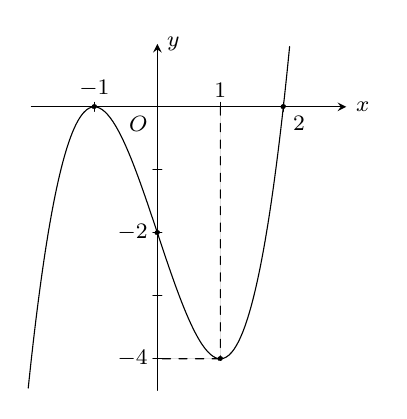
\begin{tikzpicture}[line join=round, line cap=round, >=stealth,font=\footnotesize, scale=0.8]
  \draw[->](-2,0)--(3,0) node[right] {$x$};
  \draw[->](0,-4.5)--(0,1) node[right] {$y$};
  \node (0,0) [below left]{$ O $};
  \foreach \x in {-1,...,2}
  \draw[shift={(\x,0)},color=black] (0pt,2pt) -- (0pt,-2pt);
  \foreach \y in {-4,...,0}
  \draw[shift={(0,\y)},color=black] (2pt,0pt) -- (-2pt,0pt);
  \draw[samples=100,smooth,domain=-2.05:2.1] plot (\x,{(\x+1)^2*(\x-2)});
  \draw[dashed, fill=black] (-1,0)circle(1pt) (0,-2)circle(1pt) (1,0)--(1,-4)circle(1pt) (1,-4)--(0,-4) (2,0)circle(1pt);
  \path (-1,0) node[above]{$-1$} (1,0) node[above]{$1$} (2,0) node[below right]{$2$} (0,-2) node[left]{$-2$} (0,-4) node[left]{$-4$};
 \end{tikzpicture}
 }
 \loigiai
  {
  Ta có $g'(x)=2xf'(x^2-2)$. Khi đó
  \allowdisplaybreaks
  \begin{eqnarray*}
   && f'(x^2-2)=0 \Leftrightarrow \hoac{&x^2-2=-1 \\&x^2-2=2} \Leftrightarrow \hoac{&x=\pm 1 \\&x=\pm 2.}\\
   && f'(x^2-2)>0 \Leftrightarrow x^2-2>2 \Leftrightarrow x^2>4 \Leftrightarrow \hoac{&x<-2 \\&x>2.}
  \end{eqnarray*}
  Bảng xét dấu của $g'(x)$
  \begin{center}
  
\begin{tikzpicture}
   \tkzTabInit[nocadre=false,lgt=2.5,espcl=2,deltacl=0.7] %phần bắt buộc
   {$x$/0.6, $2x$/0.6, $f'(x^2-2)$/0.6, $g'(x)$/0.6} %phần bắt buộc
   {$-\infty$, $-2$, $-1$, $0$, $1$, $2$, $+\infty$} % hàng 1 cột 2
   \tkzTabLine{,-,t,-,t,-,z,+,t,+,t,+,}
   \tkzTabLine{,+,z,-,z,-,t,-,z,-,z,+,}
   \tkzTabLine{,-,z,+,z,+,z,-,z,-,z,+,}
  \end{tikzpicture}
  \end{center}
  Vậy hàm số $g(x)=f(x^2-2)$ nghịch biến trên các khoảng $(-\infty;-2)$, $(0;2)$; đồng biến trên các khoảng $(-2;0)$, $(2;+\infty)$.
  }
\end{ex}

\begin{ex}%[Đề GHK1 môn Toán 12 THPT Việt Đức, Hà Nội, 2019-2020]%[Trần Bá Huy, dự án 12-EX-1-2020]%[2D1K1-3]
 Tìm các giá trị thực của tham số $m$ để hàm số $y=\dfrac{(m+1)x+2m+2}{x+m}$ nghịch biến trên khoảng $(-1;+\infty)$.
 \choice
  {$-1<m<2$}
  {$-1\leq m\leq 2$}
  {$m\geq 1$}
  {\True $1\leq m< 2$}
 \loigiai
  {
  Tập xác định $\mathscr{D}=\mathbb{R}\setminus\{-m\}$.\\
  Đạo hàm $y'=\dfrac{m^2-m-2}{(x+m)^2}$.\\
  Hàm số nghịch biến trên $(-1;+\infty)$ khi và chỉ khi
  \[\heva{&y'<0\\ &(-1;+\infty)\subset \mathscr{D}}\Leftrightarrow \heva{&m^2-m-2<0\\ &-m\leq -1}\Leftrightarrow\heva{&-1<m<2\\ &m\geq 1}\Leftrightarrow 1\leq m<2.\]
  }
\end{ex}

\begin{ex}%[Đề GHK1 môn Toán 12 THPT Việt Đức, Hà Nội, 2019-2020]%[Cao Thành Thái, dự án 12-EX-1-2020]%[2D1K1-3]
 Cho hàm số $y=\sin^3x+2m\sin^2x-(6+3m)\sin x+2$. Tìm số giá trị nguyên của $m$ để hàm số nghịch biến trên khoảng $\left(0;\dfrac{\pi}{2}\right)$.
 \choice
  {$3$}
  {$4$}
  {$5$}
  {\True $6$}
 \loigiai
  {
  Ta có $y'=3\sin^2 x\cos x+4m\sin x\cos x-(6+3m)\cos x = \cos x\left(3\sin^2 x+4m\sin x-6-3m\right)$.\\
  Hàm số $y=\sin^3x+2m\sin^2x-(6+3m)\sin x+2$ nghịch biến trên khoảng $\left(0;\dfrac{\pi}{2}\right)$ khi
  \[y'\leq 0, \forall x\in \left(0;\dfrac{\pi}{2}\right) \text{ và } y'=0 \text{ tại một số hữu hạn điểm thuộc } \left(0;\dfrac{\pi}{2}\right).\]
  Vì $x\in \left(0;\dfrac{\pi}{2}\right)$ nên $\cos x>0$. Ta có 
  \[y'\leq 0, \forall x\in \left(0;\dfrac{\pi}{2}\right) \Leftrightarrow 3\sin^2x+4m\sin x-6-3m\leq 0, \forall x\in \left(0;\dfrac{\pi}{2}\right).\]
  Đặt $t=\sin x$ $\Big($hàm số tăng trên $\left(0;\dfrac{\pi}{2}\right)\Big)$. Khi $x\in \left(0;\dfrac{\pi}{2}\right)$ thì $t\in(0;1)$.\\
  Ta được $y=t^3+2mt^2-(6+3m)t+2$, với $t\in(0;1)$.\\
  Ta có $y'=3t^2+4mt-6-3m$.\\
  Yêu cầu bài toán thỏa mãn khi
  \[y'\leq 0, \forall t\in(0;1) \Leftrightarrow 3t^2+4mt-6-3m\leq 0, \forall t\in(0;1).\tag{$*$}\]
  Ta có $\Delta'_{y'}=4m^2+9m+18>0,\forall m$ nên $y'=0$ luôn có hai nghiệm phân biệt $t_1$, $t_2$. Khi đó
  \[(*)\Leftrightarrow t_1\leq 0<1\leq t_2 \Leftrightarrow \heva{&3(3\cdot 0^2+4m\cdot 0-6-3m)\leq 0 \\&3(3\cdot 1^2+4m\cdot 1-6-3m)\leq 0} \Leftrightarrow \heva{&-3m-6\leq 0 \\&m-3\leq 0} \Leftrightarrow -2\leq m\leq 3.\]
  Mà $m$ là số nguyên nên $m\in\{-2;-1;0;1;2;3\}$.\\
  Vậy có $6$ giá trị nguyên của $m$ thỏa mãn yêu cầu bài toán.
  }
\end{ex}

\begin{ex}%[Đề GHK1 môn Toán 12 THPT Việt Đức, Hà Nội, 2019-2020]%[Cao Thành Thái, dự án 12-EX-1-2020]%[2D1K1-3]
 Tìm giá trị nguyên của tham số $m$ để hàm số $y=\dfrac{m^2x-4}{x-1}$ đồng biến trên từng khoảng xác định.
 \choice
  {$m=1$, $m=2$, $m=3$}
  {$m=0$, $m=1$, $m=2$}
  {\True $m=-1$, $m=0$, $m=1$}
  {$m=-2$, $m=-1$, $m=0$}
 \loigiai
  {
  Tập xác định của hàm số là $\mathscr{D}=\mathbb{R}\setminus\{1\}$.\\
  Ta có $y'=\dfrac{-m^2+4}{(x-1)^2}$.\\
  Hàm số đồng biến trên từng khoảng xác định khi $-m^2+4>0$ hay $-2<m<2$.\\
  Mà $m\in \mathbb{Z}$ nên $m\in \{-1;0;1\}$.
  }
\end{ex}

\begin{ex}%[Đề GHK1 môn Toán 12 THPT Việt Đức, Hà Nội, 2019-2020]%[Trần Bá Huy, dự án 12-EX-1-2020]%[2D1K2-5]
 Cho hàm số $y=x^4+2(m-4)x^2+m+5$ có đồ thị là $(C_m)$. Tổng các giá trị của $m$ để đồ thị $(C_m)$ có $3$ điểm cực trị tạo thành một tam giác nhận gốc tọa độ $O$ làm trọng tâm là
 \choice
  {$T=\dfrac{19}{2}$}
  {$T=\dfrac{17}{2}$}
  {\True $T=1$}
  {$T=2$}
 \loigiai
  {
  \immini
  {
  Điều kiện để hàm số có ba cực trị là 
  \[ab<0\Leftrightarrow 1\cdot 2(m-4)<0\Leftrightarrow m<4.\]
  Khi đó ba điểm cực trị $A$, $B$, $C$ của đồ thị là 
  \[A\left(0;c\right),\ B\left(-\sqrt{\dfrac{-b}{2a}};\dfrac{-\Delta}{4a}\right),\ C\left(\sqrt{\dfrac{-b}{2a}};\dfrac{-\Delta}{4a}\right).\]
  Vì $O$ là trọng tâm của $\triangle ABC$ nên
  }
  {
  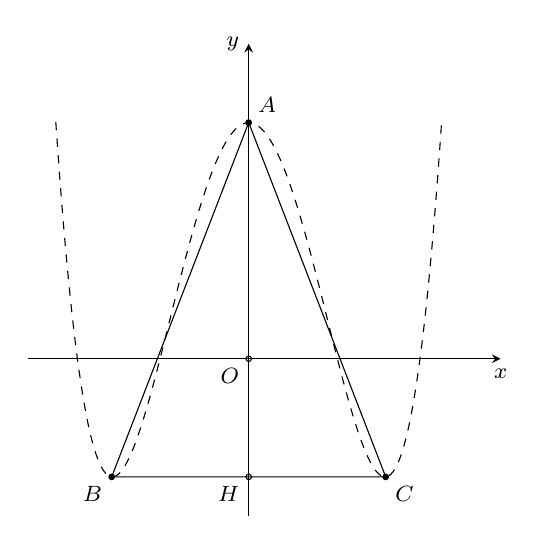
\begin{tikzpicture}[>=stealth,font=\footnotesize]
   \draw[->] (-2.8,0) -- (3.2,0) node[below] {$x$};
   \draw[->] (0,-2) -- (0,4) node[left] {$y$};
   \draw[dashed,smooth,samples=100,domain=-2.45:2.45] plot(\x,{0.5*(\x)^4-3*(\x)^2+3});
   \filldraw (0,3) circle (1pt) (-1.74,-1.5) circle (1pt) (1.74,-1.5) circle (1pt);
   \draw (0,3) node[above right] {$A$} -- (-1.74,-1.5) node[below left] {$B$} -- (1.74,-1.5) node[below right] {$C$}--(0,3);
  \draw (0,0) node[below left=-0.1] {$O$} circle (1pt) (0,-1.5) node[below left=-0.1] {$H$} circle (1pt);
  \end{tikzpicture}
  }
  \noindent
  \[c+\dfrac{-\Delta}{4a}+\dfrac{-\Delta}{4a}=0\Leftrightarrow \Delta=2ac\Leftrightarrow b^2-4ac=2ac\Leftrightarrow b^2=6ac\Leftrightarrow 4(m-4)^2=6(m+5)\Leftrightarrow \hoac{&m=1\\ &m=\dfrac{17}{2}.}\]
  Vì $m<4$ nên chỉ nhận giá trị $m=1$. Vậy $m=1$ là giá trị cần tìm, từ đó $T=1$.
  }
\end{ex}

\begin{ex}%[Đề GHK1 môn Toán 12 THPT Việt Đức, Hà Nội, 2019-2020]%[Cao Thành Thái, dự án 12-EX-1-2020]%[2D1K3-1]
 Tìm $m$ để hàm số $y=\dfrac{mx}{x^2+1}$ đạt giá trị lớn nhất tại $x=1$ trên đoạn $[-2;2]$.
 \choice
  {$m=-2$}
  {\True $m>0$}
  {$m<0$}
  {Không tồn tại $m$}
 \loigiai
  {
  Hàm số $y=\dfrac{mx}{x^2+1}$ xác định và liên tục trên đoạn $[-2;2]$.\\
  Ta có $y'=\dfrac{m\left(x^2+1\right)-mx\cdot 2x}{\left(x^2+1\right)^2} = \dfrac{-mx^2+m}{\left(x^2+1\right)^2} = \dfrac{-m\left(x^2-1\right)}{\left(x^2+1\right)^2}$.
  \begin{itemize}
   \item $m=0$ thì $y'=0$ với mọi $x\in[-2;2]$, cho nên hàm số không có giá trị lớn nhất và giá trị nhỏ nhất.
   \item $m<0$ thì $y'=0$ có nghiệm $x=\pm 1$.\\
   Bảng biến thiên của hàm số trên đoạn $[-2;2]$ là
   \begin{center}
   
\begin{tikzpicture}
    \tkzTabInit[nocadre=false,lgt=1.5,espcl=3.5,deltacl=0.7] %phần bắt buộc
    {$x$/0.6, $y'$/0.6, $y$/2} %phần bắt buộc
    {$-2$, $-1$, $1$, $2$} % hàng 1 cột 2
    \tkzTabLine{,+,z,-,z,+,}
    \tkzTabVar{-/$y(-2)$,+/$y(0)$,-/$y(1)$,+/$y(2)$}
   \end{tikzpicture}
   \end{center}
   Trường hợp này hàm số không thể đạt giá trị lớn nhất tại $x=1$.
   \item $m>0$ thì $y'=0$ có nghiệm $x=\pm 1$.\\
   Bảng biến thiên của hàm số trên đoạn $[-2;2]$ là
   \begin{center}
   
\begin{tikzpicture}
    \tkzTabInit[nocadre=false,lgt=1.5,espcl=3.5,deltacl=0.7] %phần bắt buộc
    {$x$/0.6, $y'$/0.6, $y$/2} %phần bắt buộc
    {$-2$, $-1$, $1$, $2$} % hàng 1 cột 2
    \tkzTabLine{,-,z,+,z,-,}
    \tkzTabVar{+/$y(-2)$,-/$y(0)$,+/$y(1)$,-/$y(2)$}
   \end{tikzpicture}
   \end{center}
   Để hàm số đạt giá trị lớn nhất tại $x=1$ thì
   \[y(1)>y(-2) \Leftrightarrow \dfrac{m}{2}>\dfrac{-2m}{5} \Leftrightarrow 5m>-4m \Leftrightarrow 9m>0 \Leftrightarrow m>0.\]
  \end{itemize}
  Vậy $m>0$ là giá trị thỏa mãn yêu cầu bài toán.
  }
\end{ex}

\begin{ex}%[Đề GHK1 môn Toán 12 THPT Việt Đức, Hà Nội, 2019-2020]%[Cao Thành Thái, dự án 12-EX-1-2020]%[2D1K3-6]
 Kỳ thi THPT Quốc gia năm 2018 vừa kết thúc, Nam đỗ vào trường đại học Bách Khoa Hà Nội. Hoàn cảnh không được tốt nên gia đình rất lo lắng về việc đóng học phí cho Nam. Vì vậy gia đình đã quyết định bán một phần mảnh đất hình chữ nhật có chu vi $50$ m, lấy tiền lo việc học của Nam cũng như tương lai của em. Mảnh đất còn lại sau khi bán là một hình vuông cạnh bằng chiều rộng của mảnh đất chữ nhật ban đầu. Tìm số tiền lớn nhất mà gia đình Nam nhận được khi bán đất, biết giá tiền $1$ m$^2$ đất khi bán là $1\ 500\ 000$ VNĐ.
 \choice
  {$115\ 687\ 500$ VNĐ}
  {$112\ 687\ 500$ VNĐ}
  {$114\ 187\ 500$ VNĐ}
  {\True $117\ 187\ 500$ VNĐ}
 \loigiai
  {
  \immini
  {
  Gọi $x$ (với $x>0$, đơn vị tính là mét) là chiều rộng của mảnh đất hình chữ nhật. Khi đó chiều dài của mảnh đất hình chữ nhật là $25-x$ ($0<x<25$).\\
  Chiều dài phần mảnh đất đã bán là $(25-x)-x=25-2x$.\\
  Diện tích phần mảnh đất đã bán là $x(25-2x)=25x-2x^2$.\\
  Để có được số tiền lớn nhất thì diện tích phần đất bán đi phải lớn nhất.\\
  Lại có
  \allowdisplaybreaks
  \begin{eqnarray*}
   -2x^2+25x &=& -2\left(x^2-2\cdot \dfrac{25}{4}x+\dfrac{625}{16}\right)+\dfrac{625}{8}\\
   &=& -2\left(x-\dfrac{25}{4}\right)^2+\dfrac{625}{8} \leq \dfrac{625}{8}, \forall x\in(0;25).
  \end{eqnarray*}
  }
  {
  \begin{tikzpicture}[line join=round, line cap=round, >=stealth,font=\footnotesize, scale=1]
   \draw (0,0) rectangle (2,2);
   \draw[pattern=north east lines] (0,2) rectangle (2,6);
   \draw[<->] (0,-0.2)--(2,-0.2) node[midway,below]{$x$};
   \draw[<->] (2.2,0)--(2.2,2) node[midway,right]{$x$};
  \end{tikzpicture}
  }
  \noindent
  Đẳng thức xảy ra khi $x=\dfrac{25}{4}\in(0;25)$.\\
  Vậy số tiền lớn nhất gia đình Nam nhận được là $\dfrac{625}{8}\cdot 1500000 = 117\ 187\ 500$ VNĐ.
  }
\end{ex}

\begin{ex}%[Đề GHK1 môn Toán 12 THPT Việt Đức, Hà Nội, 2019-2020]%[Cao Thành Thái, dự án 12-EX-1-2020]%[2D1K4-2]
 Có tất cả hai giá trị thực của tham số $m$ để đồ thị hàm số $y=\dfrac{x^2+m}{x^2-3x+2}$ có đúng hai đường tiệm cận. Tổng của hai giá trị của tham số $m$ đó là
 \choice
  {\True $-5$}
  {$4$}
  {$-1$}
  {$5$}
 \loigiai
  {
  Tập xác định của hàm số là $\mathscr{D}=\mathbb{R}\setminus\{1;2\}$.\\
  Ta có
  \allowdisplaybreaks
  \begin{eqnarray*}
   && \lim\limits_{x\to -\infty}y= \lim\limits_{x\to -\infty}\dfrac{x^2+m}{x^2-3x+2} = \lim\limits_{x\to -\infty}\dfrac{1+\dfrac{m}{x^2}}{1-\dfrac{3}{x}+\dfrac{2}{x^2}} = 1.\\
   && \lim\limits_{x\to +\infty}y= \lim\limits_{x\to +\infty}\dfrac{x^2+m}{x^2-3x+2} = \lim\limits_{x\to +\infty}\dfrac{1+\dfrac{m}{x^2}}{1-\dfrac{3}{x}+\dfrac{2}{x^2}} = 1.
  \end{eqnarray*}
  Vậy đồ thị hàm số $y=\dfrac{x^2+m}{x^2-3x+2}$ luôn có một đường tiệm cận ngang $y=1$.\\
  Do đó yêu cầu bài toán thỏa mãn khi và chỉ khi đồ thị hàm số $y=\dfrac{x^2+m}{x^2-3x+2}$ có đúng một tiệm cận đứng, tức là
  \[\left[\begin{aligned}&1^2+m=0 \\&2^2+m=0\end{aligned}\right. \Leftrightarrow \left[\begin{aligned}&m=-1 \\&m=-4.\end{aligned}\right.\]
  Vậy tổng hai giá trị của tham số $m$ đó là $-5$.
  }
\end{ex}

\begin{ex}%[Đề GHK1 môn Toán 12 THPT Việt Đức, Hà Nội, 2019-2020]%[Trần Bá Huy, dự án 12-EX-1-2020]%[2D1K5-3]
 Cho hàm số $y=f(x)$ thỏa mãn $f(0)=4$ và có bảng biến thiên như hình bên dưới
 \begin{center}
 
\begin{tikzpicture}[>=stealth]
  \tkzTabInit[lgt=1.5,espcl=3,deltacl=0.6]
  {$x$ /0.6, $y'$ /0.6, $y$ /2}
  {$-\infty$, $1$, $2$, $+\infty$}
  \tkzTabLine{,+,0,-,0,+,}
  \tkzTabVar{-/ $-\infty$, +/ $5$, -/ $3$, +/ $+\infty$}
 \end{tikzpicture}
 \end{center}
 Tìm tất cả các giá trị của tham số $m$ để đường thẳng $y=m$ cắt đồ thị hàm số $y=f\left(|x|\right)$ tại $6$ điểm phân biệt.
 \choice
  {\True $4<m<5$}
  {$3<m<4$}
  {$0<m<5$}
  {$3<m<5$}
 \loigiai
  {
  Từ bảng biến thiên của hàm số $y=f(x)$ suy ra bảng biến thiên của hàm số $y=f\left(|x|\right)$ như sau
  \begin{center}
  
\begin{tikzpicture}[>=stealth]
   \tkzTabInit[lgt=1.5,espcl=2,deltacl=0.6]
   {$x$ /0.6, $y'$ /0.6, $y$ /2}
   {$-\infty$, $-2$, $-1$, $0$, $1$, $2$, $+\infty$}
   \tkzTabLine{,-,0,+,0,-,0,+,0,-,0,+,}
   \tkzTabVar{+/ $+\infty$, -/ $3$, +/ $5$, -/ $4$, +/ $5$, -/ $3$, +/ $+\infty$}
  \end{tikzpicture}
  \end{center}
  Dựa vào bảng biến thiên trên suy ra đường thẳng $y=m$ cắt đồ thị hàm số $y=f\left(|x|\right)$ tại $6$ điểm phân biệt khi và chỉ khi $4<m<5$.
  }
\end{ex}

\begin{ex}%[Đề GHK1 môn Toán 12 THPT Việt Đức, Hà Nội, 2019-2020]%[Cao Thành Thái, dự án 12-EX-1-2020]%[2D1K5-6]
 Cho hàm số $y=x^3-3x^2+2x+3$ có đồ thị $(C)$. Tìm các giá trị của $m$ để qua $A(0;m)$ kẻ được đúng $3$ tiếp tuyến tới đồ thị $(C)$.
 \choice
  {\True $3<m<4$}
  {$3\leq m<4$}
  {$-1<m<5$}
  {$m\geq 4$}
 \loigiai
  {
  Ta có $y'=3x^2-6x+2$.\\
  Gọi $\Delta$ là đường thẳng đi qua $A(0;m)$ và có hệ số góc $k$. Phương trình của $\Delta$ là $y=kx+m$.\\
  Đường thẳng $\Delta$ tiếp xúc với $(C)$ khi và chỉ khi hệ sau có nghiệm
  \[\left\{\begin{aligned}&x^3-3x^2+2x+3=kx+m \\&3x^2-6x+2=k.\end{aligned}\right.\]
  Từ hệ trên suy ra
  \[x^3-3x^2+2x+3=(3x^2-6x+2)x+m \Leftrightarrow m=-2x^3+3x^2+3.\tag{$*$}\label{2GHK1-7.20-49}\]
  Xét hàm số $g(x)=-2x^3+3x^2+3$ có $g'(x)=-6x^2+6x$ và $g'(x)=0$ có các nghiệm $x=0$, $x=1$.\\
  Bảng biến thiên của hàm số $g(x)$
  \begin{center}
  
\begin{tikzpicture}
   \tkzTabInit[nocadre=false,lgt=1.5,espcl=3.5,deltacl=0.6] %phần bắt buộc
   {$x$/0.6, $g'(x)$/0.6, $g(x)$/2} %phần bắt buộc
   {$-\infty$, $0$, $1$, $+\infty$} % hàng 1 cột 2
   \tkzTabLine{,-,z,+,z,-,}
   \tkzTabVar{+/$+\infty$,-/$3$,+/$4$,-/$-\infty$}
  \end{tikzpicture}
  \end{center}
  Yêu cầu bài toán thỏa mãn khi phương trình \eqref{2GHK1-7.20-49} có ba nghiệm. Từ bảng biến thiên trên suy ra $3<m<4$ là giá trị cần tìm.
  }
\end{ex}

\begin{ex}%[Đề GHK1 môn Toán 12 THPT Việt Đức, Hà Nội, 2019-2020]%[Cao Thành Thái, dự án 12-EX-1-2020]%[2H1K3-2]
 \immini
 {
 Cho hình chóp $S.ABCD$ có $SC\perp (ABCD)$, đáy $ABCD$ là hình thoi cạnh bằng $a\sqrt{3}$ và $\widehat{ABC}=120^\circ$ (tham khảo hình vẽ). Biết rằng góc giữa hai mặt phẳng $(SAB)$ và $(ABCD)$ bằng $45^\circ$. Tính theo $a$ thể tích của khối chóp $S.ABCD$.
 \choice
  {$V=\dfrac{\sqrt{3}a^3}{12}$}
  {$V=\dfrac{3\sqrt{3}a^3}{2}$}
  {\True $V=\dfrac{3\sqrt{3}a^3}{4}$}
  {$V=\dfrac{\sqrt{3}a^3}{4}$}
 }
 {
 \begin{tikzpicture}[line join=round, line cap=round, >=stealth,font=\footnotesize, scale=0.8]
  \path (0:0) coordinate(C) (0:5) coordinate(B) (-130:2.5) coordinate(D) ($(D)+(B)-(C)$) coordinate(A) (90:4) coordinate(S);
  \draw (S)--(A)--(B)--cycle (S)--(D)--(A);
  \draw[dashed](S)--(C)--(B)--(D)--(C)--(A);
  \foreach \d/\g in {A/-40, B/0, C/180, D/-140, S/90}
  \draw[fill=black] (\d) circle(1pt) node[shift={(\g:0.3)}]{$\d$};
 \end{tikzpicture}
 }
 \loigiai
  {
  \immini
  {
  Diện tích tam giác $ABC$ là \[S_{ABC}=\dfrac{1}{2}AB\cdot BC\cdot\sin\widehat{ABC}=\dfrac{3\sqrt{3}a^2}{4}.\]
  Diện tích hình thoi $ABCD$ là \[S_{ABCD}=2S_{ABC}=\dfrac{3\sqrt{3}a^2}{2}.\]
  Ta có $(SAB)\cap (ABCD)=AB$.\\
  Kẻ $CH\perp AB$ tại $H$. Lại có $AB\perp SC$.
  }
  {
  \begin{tikzpicture}[line join=round, line cap=round, >=stealth,font=\footnotesize, scale=0.8]
   \path (0:0) coordinate(C) (0:5) coordinate(B) (-130:2.5) coordinate(D) ($(D)+(B)-(C)$) coordinate(A) (90:4) coordinate(S) ($(A)!1.4!(B)$) coordinate(H);
   \draw (S)--(A)--(B)--cycle (S)--(D)--(A) (S)--(H)--(B);
   \draw[dashed](S)--(C)--(B)--(D)--(C)--(A) (C)--(H);
   \foreach \d/\g in {A/-40, B/0, C/180, D/-140, S/90, H/0}
   \draw[fill=black] (\d) circle(1pt) node[shift={(\g:0.3)}]{$\d$};
   \tkzMarkRightAngles[size=0.2](C,H,A)
   \tkzMarkAngle[size=0.6](C,B,A)\tkzLabelAngle[pos=-1.2,rotate=10](A,B,C){$120^\circ$}
  \end{tikzpicture}
  }
  \noindent Vậy $AB\perp (SCH)$, suy ra $SH \perp AB$.\\
  Do đó góc giữa hai mặt phẳng $(SAB)$ và $(ABCD)$ bằng góc giữa $SH$ và $CH$, chính là $\widehat{SHC}=45^\circ$.\\
  Ta có $CH=\dfrac{2S_{ABC}}{AB} = \dfrac{3\sqrt{3}a^2}{2\cdot a\sqrt{3}} = \dfrac{3a}{2}$.\\
  Tam giác $SCH$ vuông cân tại $C$ nên $SC=CH=\dfrac{3a}{2}$.\\
  Thể tích của khối chóp $S.ABCD$ là $V=\dfrac{1}{3}S_{ABCD}\cdot SC = \dfrac{1}{3}\cdot \dfrac{3\sqrt{3}a^2}{2}\cdot \dfrac{3a}{2} = \dfrac{3\sqrt{3}a^3}{4}$.
  }
\end{ex}

\begin{ex}%[Đề GHK1 môn Toán 12 THPT Việt Đức, Hà Nội, 2019-2020]%[Cao Thành Thái, dự án 12-EX-1-2020]%[2H1K3-2]
 \immini
 {
 Cho hình chóp $S.ABCD$ có đáy $ABCD$ là hình thang vuông tại $A$ và $D$ (tham khảo hình vẽ). Biết $AB=AD=2a$, $CD=a$. Gọi $I$ là trung điểm của $AD$, biết hai mặt phẳng $(SBI)$ và $(SCI)$ cùng vuông góc với mặt phẳng $(ABCD)$. Góc giữa hai mặt phẳng $(SBC)$ và $(ABCD)$ bằng $60^\circ$. Tính thể tích của khối chóp $S.ABCD$.
 \choice
  {\True $V=\dfrac{3\sqrt{15}a^3}{5}$}
  {$V=\dfrac{3\sqrt{5}a^3}{8}$}
  {$V=\dfrac{3\sqrt{5}a^3}{5}$}
  {$V=\dfrac{3\sqrt{15}a^3}{8}$}
 }
 {
 \begin{tikzpicture}[line join=round, line cap=round, >=stealth,font=\footnotesize, scale=0.6]
  \path (0:0) coordinate(A) (0:5) coordinate(B) (-130:3.5) coordinate(D)+(0:2.5) coordinate(C) ($(A)!.5!(D)$) coordinate(I)+(90:5) coordinate(S);
  \draw (S)--(B)--(C)--cycle (S)--(D)--(C);
  \draw[dashed](S)--(A)--(B) (D)--(A);
  \foreach \d/\g in {A/60, B/0, C/-40, D/-140, S/90, I/180}
  \draw[fill=black] (\d) circle(1pt) node[shift={(\g:0.3)}]{$\d$};
 \end{tikzpicture}
 }
 \loigiai
  {
  \immini
  {
  Ta có
  \[\heva{&(SBI)\perp (ABCD) \\&(SCI)\perp (ABCD) \\&(SBI)\cap (SCI)=SI} \Rightarrow SI\perp (ABCD).\]
  Gọi $M$ là trung điểm của $AB$. Khi đó $ADCM$ là hình chữ nhật.\\
  Tam giác $ICD$ vuông tại $D$ nên $IC=\sqrt{ID^2+DC^2}=a\sqrt{2}$.
  }
  {
  \begin{tikzpicture}[line join=round, line cap=round, >=stealth,font=\footnotesize, scale=0.70]
   \path (0:0) coordinate(A) (0:5) coordinate(B) (-127:3.5) coordinate(D)+(0:2.5) coordinate(C) ($(A)!.5!(D)$) coordinate(I)+(90:5) coordinate(S) ($(A)!.5!(B)$) coordinate(M) ($(C)!.3!(B)$) coordinate(H);
   \draw (S)--(B)--(C)--cycle (H)--(S)--(D)--(C);
   \draw[dashed](I)--(S)--(A)--(B) (D)--(A)--(C)--(M) (C)--(I)--(B) (I)--(H);
   \foreach \d/\g in {A/60, B/80, C/-40, D/-100, S/90, I/180, M/90, H/-40}
   \draw[fill=black] (\d) circle(1pt) node[shift={(\g:0.3)}]{$\d$};
   \tkzMarkRightAngles[size=0.2](I,H,C)
  \end{tikzpicture}
  }
  \vspace*{0.2cm}
  \noindent
  Tam giác $IAB$ vuông tại $A$ nên $IB=\sqrt{IA^2+AB^2}=a\sqrt{5}$.\\
  Tam giác $BCM$ vuông tại $M$ nên $BC=\sqrt{BM^2+CM^2}=a\sqrt{5}$.\\
  Kẻ $IH\perp BC$ tại $H$, lại có $BC\perp SI$ nên $BC\perp (SIH)$, suy ra $BC\perp SH$.\\
  Mặt khác $(SBC)\cap (ABCD)= BC$.\\
  Cho nên góc giữa hai mặt phẳng $(SBC)$ và $(ABCD)$ bằng góc giữa $IH$ và $SH$, chính là $\widehat{SHI}$.\\
  Diện tích tam giác $IBC$ là
  \[S_{IBC}=\sqrt{p(p-IB)(p-IC)(p-BC)} = \dfrac{3a^2}{2}, \text{ với } p=\dfrac{IB+IC+BC}{2}=\dfrac{\left(2\sqrt{5}+\sqrt{2}\right)a}{2}.\]
  Suy ra $IH=\dfrac{2S_{IBC}}{BC} = \dfrac{3a^2}{a\sqrt{5}} = \dfrac{3\sqrt{5}a}{5}$.\\
  Trong tam giác $SIH$ vuông tại $I$ ta có
  \[\tan\widehat{SHI}=\dfrac{SI}{IH} \Rightarrow SI=IH\cdot \tan\widehat{SHI} = \dfrac{3\sqrt{15}a}{5}.\]
  Diện tích hình thang $ABCD$ là $S_{ABCD}=\dfrac{(AB+CD)AD}{2} = \dfrac{(2a+a)\cdot 2a}{2} = 3a^2$.\\
  Thể tích của khối chóp $S.ABCD$ là $V=\dfrac{1}{3}S_{ABCD}\cdot SI = \dfrac{1}{3}\cdot 3a^2\cdot \dfrac{3\sqrt{15}a}{5} = \dfrac{3\sqrt{15}a^3}{5}$.
  }
\end{ex}

\Closesolutionfile{ans}
\begin{indapan}{10}
	{ans/ans-2-GHK1-7-VietDuc-HaNoi-20}
\end{indapan}
